\documentclass[pdflatex,sn-mathphys-num]{sn-jnl}


\theoremstyle{thmstyleone}
\newtheorem{theorem}{Theorem}
\newtheorem{proposition}[theorem]{Proposition}
\theoremstyle{thmstyletwo}
\newtheorem{remark}{Remark}
\theoremstyle{thmstylethree}
\newtheorem{definition}{Definition}

\usepackage{graphicx}
\usepackage{multirow}
\usepackage{amsmath,amssymb,amsfonts}
\usepackage{mathtools}
\usepackage{booktabs}
\usepackage{xcolor}
\usepackage{algorithm}
\usepackage{algorithmicx}
\usepackage{algpseudocode}
\usepackage{tikz}
\usetikzlibrary{arrows.meta,positioning}

% sn-mathphys-num.bst emits \burl for URLs and falls back to \textsf (which
% breaks on underscores) when \burl is undefined; route it through hyperref.
\providecommand{\burl}[1]{\url{#1}}

\graphicspath{{figures/}}

\newcommand{\vI}{\textcolor[rgb]{0.11,0.60,0.36}{\textbf{I}}}
\newcommand{\vR}{\textcolor[rgb]{0.80,0.16,0.16}{\textbf{R}}}
\newcommand{\vU}{\textcolor[rgb]{0.85,0.55,0.00}{\textbf{U}}}
\newcommand{\F}{\mathcal{F}}
\newcommand{\G}{\mathcal{G}}
\newcommand{\Ucal}{\mathcal{U}}
\newcommand{\KL}{\mathrm{KL}}
\newcommand{\Bern}{\mathrm{Bern}}
\newcommand{\eps}{\varepsilon}
\newcommand{\Efrak}{\mathbb{E}}

\raggedbottom

\begin{document}

\title[Anytime-Valid Certificates for Machine Unlearning]{VOUCH: Anytime-Valid Certificates for Machine Unlearning via Paired-Canary Hypothesis-Betting}

% Double-blind toggle: \anontrue for the review copy (author identity moves to
% the cover letter); \anonfalse for the camera-ready version.
\newif\ifanon
\anontrue

\ifanon
\author*[1]{\sur{Anonymous Author}}
\affil*[1]{\orgname{Blinded for double-blind review}}
\else
\author*[1]{\fnm{Quang-Vinh} \sur{Dang}}\email{vinh.dq4@buv.edu.vn}
\affil*[1]{\orgname{British University Vietnam}, \orgaddress{\city{Hung Yen}, \country{Vietnam}}}
\fi

\abstract{Machine unlearning methods for large language models are deployed to honour
deletion requests, yet they ship with no statistical certificate that forgetting
occurred. The evaluations in common use are fixed-sample tests: unsound as membership
evidence unless what enters training is randomised, void the moment an auditor
inspects evidence as it accumulates, and dependent on a retrained reference that is
unaffordable at scale and ill-defined for multi-stage pipelines. We introduce
\emph{VOUCH}, an anytime-valid certification framework. At fine-tuning time the
provider plants \emph{paired ghost canaries}: exchangeable twin records of which a
fair coin admits one into training, and later into the forget set, while the other is
never shown to any model. Exact unlearning leaves the twins interchangeable, so the
within-pair score difference is symmetric \emph{by construction}, giving an exact,
distribution-free, finite-sample null that needs no shadow models, no retrained
reference, and no assumption about the model. Betting e-processes over this null yield
three coupled objects: an anytime-valid confidence sequence on the residual membership
advantage, an $(\eps,\alpha)$-forgetting certificate from sequential two-sided
equivalence testing, and a revocation alarm. Because every canary passes through one
jointly trained model its signs are dependent, so we certify the \emph{realised
advantage on the committed cohort} and bet against a without-replacement boundary,
which is exact under arbitrary dependence; the marginal alternative is breached
eightfold under model-level over-dispersion. Certificates and alarms provably compose
in opposite directions---by consensus and by product. Across a 2{,}000-seed
calibration study, four valid sequential comparators, and TOFU and MUSE-News over six
architectures from 0.9M to 5.1B parameters, VOUCH certifies exact unlearning down to
$\eps = 0.05$, revokes un-unlearned models within a handful of pairs, and exposes
gradient ascent that forgets by destroying the model, at $2Qm$ forward passes and no
training. The certificate concerns a declared score class on a committed cohort under
an honest-but-verifiable provider, and we measure what each qualification costs.}

\keywords{machine unlearning, anytime-valid inference, e-values, membership inference,
certification, large language models}

\maketitle

\section{Introduction}\label{sec:intro}

When a user invokes the right to erasure, a model provider must do more than run an
unlearning routine: it must be able to \emph{show}, to a regulator or an internal audit
function, that the routine worked. This obligation is concrete, though it is worth
locating it precisely. Article~17 of the GDPR creates the right to erasure itself, but
the duty to \emph{demonstrate} rather than merely assert compliance lives in
Articles~5(2) and 24(1), which require controllers to be able to show that processing
conforms to the Regulation, and in Article~58(1)(b), which empowers supervisory
authorities to conduct data-protection audits \citep{gdpr2016}. The EU AI Act adds
obligations of a different shape: automatic event logging over a system's lifetime
(Article~12), technical documentation and its ten-year retention (Articles~11 and 18),
production of that documentation and those logs to authorities on reasoned request
(Article~21), conformity assessment (Article~43), and the AI Office's power to evaluate
general-purpose models (Article~92) \citep{aiact2024}. Neither instrument prescribes a
statistical test for erasure. Both presuppose that a provider can produce evidence, and
that is the gap this paper addresses.

The algorithmic side of machine unlearning has risen to meet the demand: gradient ascent
and its stabilised successors, negative preference optimisation
\citep{zhang2024npo,fan2025simnpo}, representation misdirection \citep{li2024wmdp},
and task-vector negation now remove targeted knowledge from large models at modest
cost. The \emph{verification} side has not kept pace, and a substantial recent
literature documents why: forget-quality metrics track surface behaviour rather than
retained knowledge and collapse under attack \citep{wang2025towards}, output-matching
scores hide degenerate models \citep{yuan2025closer}, benign relearning on unrelated
public text restores supposedly erased content \citep{hu2025jogging}, and
gradient-ascent objectives redistribute probability mass onto paraphrases so that
standard metrics report success while the information remains
\citep{li2026beliefs,feng2025existing}. Evaluation, not optimisation, is the bottleneck.

\paragraph{Three obstacles.} Three specific obstacles stand between current practice
and a defensible certificate. \emph{First}, a high membership-inference score on a
supposedly forgotten example is not evidence that the example was ever trained on.
Distribution shift and the model's own priors confound the signal, and
\citet{zhang2024mia} have shown formally that membership cannot be established without
controlling the randomness of what enters training. \emph{Second}, deletion requests
arrive as a stream and auditors inspect the evidence as it accrues, stopping when they
are satisfied; every fixed-sample test in current use---the forget-quality metric of
\citet{maini2024tofu}, the leakage metric of \citet{shi2024muse}, the shadow-model
panels of \citet{hayes2024inexact}---has its error guarantee voided by exactly this
optional stopping, and we measure the damage in Section~\ref{sec:exp-validity}.
\emph{Third}, the comparators these tests rely on---a model retrained from scratch
without the deleted data---are prohibitively expensive at the scale of modern language
models and, as \citet{yu2025impossibility} show, are not even well defined for the
multi-stage pipelines used in practice, because path-dependence means no unique
retrained model exists to compare against.

\paragraph{The design.} VOUCH addresses all three with a single design decision and a
single inferential engine. The design decision is the \emph{paired ghost canary}. At
fine-tuning time we generate exchangeable twin records, and for each pair we flip a
fair coin to decide which twin is admitted into training; the admitted twin is later
appended to the forget set, so that it passes through the very same unlearning pipeline
as organic data, while its twin is withheld from every model. This construction is what
makes the audit sound: under exact unlearning the model is independent of the coin, so
the two twins are exchangeable and the difference between their scores is symmetric
about zero \emph{regardless of the model, the scoring function, or the data
distribution}. We therefore obtain an exact, distribution-free, finite-sample null that
we generated ourselves, rather than one we must assume. The engine is the betting
e-process from game-theoretic statistics, which turns this null into a test whose
validity holds not at one predetermined sample size but at every stopping time at once,
by Ville's inequality. Streaming deletions and continuous public monitoring, fatal to a
fixed-sample test, are precisely what an e-process is built to survive.

\paragraph{What the certificate claims, and what it does not.} We state the scope here
because it governs how every later number should be read, and because a certificate
whose scope is overclaimed is worse than none. A VOUCH certificate asserts that the
residual advantage extractable by a \emph{declared class $\F$ of scores}, on the
\emph{committed canary cohort}, against the \emph{deployed model}, is below a declared
tolerance $\eps$, under an \emph{honest-but-verifiable} provider who genuinely executes
the unlearning routine on the forget set as declared. Four qualifications follow, and
each is quantified rather than merely disclosed. The guarantee is per-cohort, not
per-deletion-request, since per-request certificates would need per-user canaries. It
concerns $\F$, and Section~\ref{sec:exp-outclass} exhibits an attack from outside $\F$
that exceeds the tolerance on $3.2\%$ of certified runs. The transfer from the realised
cohort to the algorithm-level advantage costs an explicit inflation of
$\kappa\sqrt{2\log(2/\alpha')/m}$ (Proposition~\ref{prop:transfer}), which is why our
tight-tolerance results are cohort statements. And the honest-but-verifiable assumption
is load-bearing in a way we had underestimated:
Section~\ref{sec:exp-detect} shows a zero-knowledge perplexity filter recovers the
entire planted cohort, so a provider who wished to special-case it could find it, and
only cryptographic attestation \citep{eisenhofer2025verifiable} closes that gap. What
detection does not do is defeat the audit, because both twins in a pair are equally
conspicuous and locating the cohort reveals nothing about which twin the coin admitted.

\paragraph{Corrections carried by this version.} Building the framework and running it
end-to-end forced five corrections on the initial design, and because each turned out
to matter we foreground them rather than bury them. \emph{(i)} The certificate's null
must be stated conditionally, not marginally. Signs from all canaries pass through one
jointly trained model, so they are dependent; a fixed-boundary process that assumes
otherwise is breached eightfold under model-level over-dispersion
(Table~\ref{tab:dependence}). We retarget the certificate at the realised cohort
advantage and bet against a without-replacement boundary, which is exact under
arbitrary dependence (Theorem~\ref{thm:cert}). \emph{(ii)} The natural way to combine
several attack scores into one certificate---bet on an adaptively weighted mixture of
their signs---is \emph{anytime-invalid}, and in simulation our own earlier design
falsely certified a leaking model $99.6\%$ of the time; the sound alternative requires
every score's own process to concur. \emph{(iii)} Certificates and alarms must compose
in \emph{opposite} directions across deletion waves, and multiplying certificate
e-values, the instinctive move, certifies histories that contain a genuinely bad wave.
\emph{(iv)} Gradient-ascent unlearning frequently \emph{over-forgets} on real language
models, driving the forgotten twins to scores conspicuously \emph{below} their
never-seen partners---membership leakage that a one-sided test happily certifies and
that a two-sided test must catch. \emph{(v)} The small-$\eps$ expansion of the
Kullback--Leibler drift is $\eps^2/2$, not $\eps^2/8$, so the cohort-size rule is
$2\log(1/\alpha)/\eps^2$; the numerical columns were always computed from the exact
divergence and are unaffected, but the stated rule was wrong by a factor of four.

\paragraph{Contributions.} We formulate unlearning certification as sequential
two-sided equivalence testing against a declared attack class, with an exact
distribution-free null supplied by paired ghost canaries
(Section~\ref{sec:framework}). We give the supporting theory: an exact conditional null
requiring no independence across pairs, a certificate that is exact under arbitrary
dependence via without-replacement betting, a priced bridge to the super-population
advantage, sound composition across scores and across deletion waves in both
directions, power that matches the Kullback--Leibler information limit, and a
one-directional consistency bridge from certified $(\eps_u,\delta_u)$-unlearning
(Section~\ref{sec:theory}). We report a comprehensive empirical study
(Section~\ref{sec:exp}): calibration under adversarial optional stopping over 2{,}000
seeds; head-to-head comparison against four \emph{valid} sequential procedures;
end-to-end certification of gradient ascent, GradDiff, NPO, SimNPO, and retraining on
TOFU and MUSE-News across three architectures with a tolerance sweep down to
$\eps = 0.05$, utility guardrails, and dose--response calibration; a head-to-head
against the descriptive metrics VOUCH is argued to replace; attacks from outside the
declared score class; a measurement of how detectable the planted cohort is, with an
entropy-dilution design rule that follows from it; recoverability probes that relearn,
quantise, and jailbreak the unlearned model; a model axis spanning 2019 to 2026; and
cost measurements with their hardware and workload assumptions stated. All code, all
results, and the fault-tolerant harness that produced them on free ephemeral compute
are released.

\section{Related work}\label{sec:related}
Our work sits at the meeting point of four literatures---unlearning algorithms, the
measurement of memorisation and forgetting, the verification of unlearning, and
game-theoretic statistics---and it is the gap between the middle two that
game-theoretic statistics turns out to close. We survey each in turn and then state
precisely how VOUCH differs from its nearest neighbours.

\subsection{Unlearning algorithms and their benchmarks}

Exact unlearning by architectural design, exemplified by sharded training
\citep{bourtoule2021machine}, retrains only the shards touched by a deletion; it is
sound but cannot be applied to a model that was not trained for it, which is the
situation every deployed language model is in. The practical response has therefore
been \emph{approximate} unlearning, and for large language models a compact toolbox
has emerged: gradient ascent on the forget set and its retain-regularised variant
GradDiff; negative preference optimisation \citep{zhang2024npo}, which replaces the
unbounded ascent objective with a bounded preference loss and which its authors
introduced precisely to avoid the catastrophic collapse that ascent invites; the
simplified reappraisal SimNPO \citep{fan2025simnpo}, which discards NPO's frozen
reference model in favour of a length-normalised margin objective and which we
include as a subject in Section~\ref{sec:exp-bench}; representation misdirection
\citep{li2024wmdp}, which acts on hidden activations rather than on the token loss and
which we add as a subject in Section~\ref{sec:exp-rmu}; and task-vector negation. These methods are evaluated on
purpose-built benchmarks---TOFU's fictitious-author question answering
\citep{maini2024tofu}, MUSE's six-way news-and-books evaluation \citep{shi2024muse},
and the hazardous-knowledge multiple-choice of WMDP \citep{li2024wmdp}---and we treat
all of them, methods and benchmarks alike, as \emph{subjects} that VOUCH certifies
rather than as competitors.

\subsection{Measuring memorisation and forgetting}

The canary methodology VOUCH depends on descends directly from the secret-sharer line
of work. \citet{carlini2019secret} insert random secret sequences into training data
and define \emph{exposure}, the canary's rank among all possible instantiations
ordered by model log-perplexity, converting memorisation into a calibrated number;
they show that memorisation is commonplace, that it is not explained by overfitting,
and that it is eliminated only by differentially private training. VOUCH borrows the
planted-canary device and changes one thing that turns out to matter for inference:
where the secret sharer plants a canary and \emph{measures} its exposure, we plant a
\emph{pair} and randomise which twin enters training, so that the measurement acquires
a null. Exposure answers ``how memorised is this string''; the ghost twin answers
``could this have happened by chance,'' which is the question a certificate must
answer and the one \citet{zhang2024mia} show cannot be answered without controlled
randomisation.

The strongest membership attacks in this lineage calibrate per example rather than
thresholding a raw score. \citet{carlini2022lira} show that comparing a target model's
confidence on an example against the confidences that shadow models trained with and
without it produce---a likelihood-ratio test they call LiRA---dominates score-threshold
attacks, particularly in the low false-positive regime that matters for a privacy
claim. LiRA is the natural adversary against which to stress-test a declared score
class, since it uses information no member of ours has: $N$ additionally trained
models. It is for the same reason not a candidate for inclusion in $\F$, because a
verifier held to $2Qm$ forward passes and no training cannot run it. We use it in
Section~\ref{sec:exp-lira} as an attack from outside the class, with a positive
control that establishes it is working before its null on a certified model is read as
meaning anything.

The complementary literature measures forgetting rather than memorisation.
\citet{jagielski2023measuring} quantify how the success of privacy attacks on a
training example decays as training continues past it, and find that standard models
do forget over time---but also prove that non-convex models can retain memorised data
indefinitely, and show that forgetting disappears entirely under deterministic
training. Their conclusion is the premise of ours: incidental forgetting is real but
uncontrolled, and therefore cannot substitute for a certificate.
\citet{barbulescu2024each} document, in the same spirit, how per-sequence memorisation
strength governs how hard a datum is to remove, which is the phenomenon our
repetition strata are designed to traverse.

\subsection{Evaluating unlearning: a literature of negative results}

What the unlearning literature has increasingly documented is that the metrics used
to declare success are unreliable, and this body of work is the direct motivation for
VOUCH. A first strand shows that apparent forgetting is often mere suppression.
\citet{lucki2024adversarial} recover ostensibly unlearned capabilities through
lightweight attacks; \citet{zhang2025quantization} show that quantising an unlearned
model to $4$ bits resurrects forgotten knowledge; \citet{deeb2024remove} recover most
pre-unlearning accuracy by fine-tuning on adjacent facts; and \citet{fan2025relearning}
formalise relearning attacks and connect robustness to sharpness-aware minimisation.
Closest to our P1 probe is \citet{hu2025jogging}, who show that fine-tuning an
unlearned model on a small, \emph{benign}, publicly available corpus that never
contains the forget targets is enough to jog the model's memory and restore both
hazardous knowledge and verbatim memorised passages. Their framing---obfuscation
versus removal---is precisely the distinction our relearn probe operationalises, and
their result is why we treat a post-relearning verdict as part of the certificate
rather than as an optional extra: on our benchmark tier at $\eps = 0.2$ the same probe
revokes NPO's certificate on one MUSE/GPT-2 seed and one MUSE/Phi-1.5 seed, and leaves
it intact on every TOFU cell (Section~\ref{sec:exp-bench}).

A second strand indicts the evaluation protocols themselves.
\citet{feng2025existing} demonstrate that current LLM-unlearning evaluations can be
made to both overstate and understate success. \citet{wang2025towards} show that
forget-quality metrics track surface output behaviour rather than retained knowledge
and collapse under red-teaming, and---more damagingly for cross-paper
comparison---that the reported unlearning/retention trade-off does not lie on a Pareto
frontier, so method rankings are artifacts of hyperparameter choice; they propose
recalibrating retained performance before comparing. \citet{yuan2025closer} make the
complementary point that ROUGE-style output matching hides degenerate behaviour, and
add metrics for token diversity, sentence semantics, and factual correctness. Both
diagnoses apply to VOUCH's subjects and shaped how we report them: we do not rank
unlearning methods against one another, we certify each one against a declared
tolerance and pair every verdict with a utility reading, precisely because a ranking
built on a non-Pareto trade-off would not survive a change of hyperparameters. Our own
worked example in Figure~\ref{fig:example} is an instance of the degeneracy
\citet{yuan2025closer} warn about---an NPO-unlearned model emitting
\texttt{LLLLLL\ldots} on canary prompts while its held-out loss is untouched---and it
is caught here not by a fluency metric but by the two-sided certificate, which treats
scoring conspicuously \emph{below} the ghost twin as leakage.

A third strand is mechanistic and, for our purposes, the most pointed.
\citet{wei2025forget} show that facts presumed forgotten persist through correlated
knowledge, and \citet{xu2026reversibility} distinguish genuine erasure from
suppression at the representation level, finding behaviour easily restored by minimal
fine-tuning. \citet{li2026beliefs} identify the mechanism they call the
\emph{squeezing effect}: gradient-ascent-style objectives push probability mass off
the target response but redistribute it onto nearby high-likelihood regions, typically
semantically equivalent rephrasings, so the content resurfaces under paraphrase and
commonly used metrics report success while semantically related information remains.
Their remedy couples the unlearning objective to the model's own high-confidence
generations. This result bears directly on the scope of what VOUCH certifies and we
want to be exact about the relationship. VOUCH is a \emph{verification} framework and
inherits the limits of its declared score class: our scores read the likelihood of the
literal secret span under a fixed set of query wrappers, so probability mass that has
migrated to a paraphrase is, by construction, mass our default class does not see. The
framework's response is structural rather than rhetorical---the class $\F$ is declared,
the certificate is explicitly a statement about $\F$, and any score a sceptic can name
can be added to $\F$ at the cost of a slower certificate and no loss of validity, since
Theorem~\ref{thm:cert} needs no multiplicity correction. Sections~\ref{sec:exp-outclass} and
\ref{sec:exp-lira} run attacks from \emph{outside} the declared class against
already-certified models and report where they exceed the tolerance. We also
implement the score their result calls for: Section~\ref{sec:exp-para} adds a
paraphrase-aware member to $\F$, which costs one to two per cent in pairs and changes
no verdict---though we are explicit there that our random-string secrets have no
semantic neighbourhood for mass to migrate into, so this tests the score's cost rather
than the squeezing effect itself, which would need canaries whose secret is
paraphrasable.

The recurring message across all of this is that \emph{evaluation}, not optimisation,
is the bottleneck---which is exactly the problem VOUCH addresses, and which motivates
our recoverability probes (R-VOUCH) and our insistence on pairing every certificate
with a utility reading.

\subsection{Verifying and certifying unlearning}

The earliest guarantees came from \emph{certified removal}
\citep{guo2020certified,sekhari2021remember,neel2021descent,ginart2019making}, which
bounds the distance between the unlearned and retrained models in a differential-
privacy-style $(\eps_u,\delta_u)$ sense. These results are elegant but confined to
convex or near-convex regimes, and their bounds become vacuous at the scale of modern
language models; we use them not as a baseline but as a consistency check, showing in
Proposition~\ref{prop:bridge} that any $(\eps_u,\delta_u)$-certified algorithm passes
VOUCH---a one-directional implication, as Remark~\ref{rem:onedirection} states.
The verification of \emph{arbitrary} unlearning has proven far harder.
\citet{thudi2022necessity} argue that approximate unlearning cannot be audited from
weights alone and that auditable definitions are a prerequisite for any guarantee;
\citet{zhang2024verification} show that a dishonest provider can defeat both existing
families of verification strategies while passing them; and, most consequentially for
our design, \citet{zhang2024mia} establish that membership-inference scores
\emph{cannot} prove that a model was trained on given data unless the inclusion of
that data was randomised---the soundness principle that our fair-coin canary design
is built to satisfy. Two further impossibility results bound what any behavioural
certificate can claim: \citet{yu2025impossibility} show that path-dependence makes
retrain equivalence unattainable for multi-stage pipelines, which is why VOUCH's null
is internally generated rather than referenced to a retrained model, and the
reversibility findings above imply that no behavioural method can certify
parameter-space erasure---a limit we state explicitly rather than paper over.

A handful of recent efforts move toward statistical certification, and these are our
closest neighbours. \citet{pandey2025gaussian} give a hypothesis-testing notion of
certified unlearning, but it is fixed-sample and tied to a Gaussian high-dimensional
regression regime rather than to LLM-scale behavioural auditing.
\citet{pawelczyk2025machine} use data-poisoning as a lens on unlearning failure but
provide no error-controlled certificate. Cryptographic proof-of-unlearning
\citep{eisenhofer2025verifiable} attests that the correct computation \emph{ran},
which is orthogonal to whether forgetting \emph{holds} statistically and with which
VOUCH composes---and which is the right tool against the special-casing provider our
threat model excludes. The recent survey of \citet{xue2026survey} organises this
fast-moving area and confirms that no existing method delivers what VOUCH does: an
anytime-valid, distribution-free certificate of bounded residual influence. The
broader programme is surveyed by \citet{liu2025rethinking}.

\subsection{Game-theoretic statistics}

The inferential engine we borrow is that of safe, anytime-valid inference: e-values,
test martingales, and betting confidence sequences
\citep{ramdas2023game,grunwald2024safe,shafer2021testing,waudbysmith2024,howard2021time}.
The defining property, traceable to Ville's inequality \citep{ville1939}, is that a
nonnegative martingale started at one exceeds $1/\alpha$ with probability at most
$\alpha$ \emph{at every stopping time simultaneously}; this is precisely what a
streaming, continuously-monitored deletion audit requires, and precisely what a
fixed-sample test cannot offer. The betting perspective
\citep{waudbysmith2024,orabona2016coin} additionally supplies confidence sequences
whose bets adapt online to near-optimal growth, and---the ingredient our corrected
certificate turns on---the without-replacement construction for finite-population
means, in which the null boundary is recentred at each step on the mean the unsampled
remainder would need to carry. That device is what lets Theorem~\ref{thm:cert} dispense
with independence across pairs entirely. The one adjacent application of these tools
is to privacy auditing: \citet{steinke2023privacy} audit differential
privacy in a single training run, and \citet{gonzalez2025sequential} and
\citet{csillag2026dpevalues} bring sequential e-value machinery to DP auditing. The
distinction is fundamental to the hypothesis structure. Privacy auditing
\emph{lower}-bounds the privacy loss of a \emph{training} algorithm by mounting a
successful attack; VOUCH \emph{upper}-bounds the residual influence \emph{after
unlearning} by showing that no attack in a declared class succeeds---an equivalence
test, not a significance test, run over ghost twins that have passed through the
unlearning pipeline. To our knowledge, VOUCH is the first application of
game-theoretic statistics to unlearning certification.

\subsection{Positioning}

The contrast with our nearest neighbours can be summarised sharply. Fixed-sample
paired or two-sample tests---including the KS-based forget-quality metric of
\citet{maini2024tofu} and the min-$k\%$ leakage metric of \citet{shi2024muse}---are
invalidated by optional stopping and typically require a retrained reference;
Section~\ref{sec:exp-descriptive} runs both on our own models and seeds and reports
where they and VOUCH disagree. The sound-membership results of \citet{zhang2024mia}
tell us \emph{why} controlled randomness is indispensable but stop at a fixed-$n$
membership proof rather than a sequential forgetting certificate; the secret-sharer
and forgetting-measurement lines \citep{carlini2019secret,jagielski2023measuring}
supply the canary device and the decay measurements but no null and no error control;
shadow-model evaluators \citep{hayes2024inexact} are descriptive and cost dozens of
fine-tunes; certified removal \citep{guo2020certified,sekhari2021remember} does not
scale; and DP auditing \citep{steinke2023privacy,gonzalez2025sequential} solves the
opposite, lower-bounding, problem. VOUCH is, to our knowledge, the first framework to
formulate unlearning certification as sequential equivalence testing and to deliver
exact, finite-sample, anytime-valid certificates of bounded residual influence at LLM
scale, with soundness inherited from a randomised paired-canary design rather than
from distributional assumptions or shadow models.


\section{Setting and the VOUCH protocol}\label{sec:framework}
This section develops the protocol in full: the actors and threat model, the canary
construction that manufactures the null, the filtration that makes the martingale
argument literally correct, the certified quantity, the betting engine with its
explicit wealth dynamics, and finally the assembled protocol as pseudocode
(Algorithm~\ref{alg:vouch}) and as a flowchart (Figure~\ref{fig:flowchart}).

\subsection{Actors, pipeline, and threat model}\label{sec:setting}

The provider fine-tunes a base model on
$D_{\text{keep}} \cup D_{\text{forget}} \cup C$, where $C$ is the canary set described
below. When deletion requests arrive, an unlearning algorithm $\Ucal$---negative
preference optimisation, GradDiff, and so on---produces an unlearned model $M_u$ from
the fine-tuned model, using the forget set augmented with the relevant canaries. A
verifier, holding only black-box query access to $M_u$ together with a canary manifest
whose commitment was published before unlearning began, runs VOUCH and either issues,
withholds, or revokes a certificate.

Throughout we assume the \emph{honest-but-verifiable} setting: the provider genuinely
executes $\Ucal$ on the forget set as declared, and the open question is whether it
worked and how well, under quantified error control. This assumption is doing real
work and we state it wherever the certification claim is summarised, because the
commitment prevents the manifest from being changed after the fact but does not
prevent a provider who has \emph{located} the cohort from treating it differently
from organic data. Section~\ref{sec:exp-detect} measures how hard locating the cohort
actually is---the answer is: much easier than we had assumed---and explains why
locating it is nonetheless not the same as defeating the audit: both twins in a pair
are equally conspicuous, so a provider who finds the cohort still learns nothing
about which twin the coin admitted. A provider willing to special-case the committed
canaries is outside our scope and, as prior work establishes, can only be addressed
by cryptographic attestation \citep{eisenhofer2025verifiable}, with which VOUCH
composes.

\subsection{Paired ghost canaries}\label{sec:canaries}

A templated generator emits exchangeable twin pairs
$(c_i^0, c_i^1)$ for $i = 1,\dots,m$. The two twins in a pair are independent draws from
the same conditional template distribution---the same surface form populated with
independently sampled fictitious entities carrying secrets of at least $40$ bits of
entropy---so that within a pair they are exchangeable by construction. We match the
template to the host corpus, using question--answer pairs for TOFU and record-style
sentences for news text. For each pair an
independent fair coin $b_i \sim \Bern(\tfrac12)$ selects the \emph{in-twin}
$c_i^{b_i}$, which we insert into
the fine-tuning corpus with a repetition factor $r_i \in \{1,2,4,8\}$ (these strata give
us a dose--response curve) and later append to the forget set, so that it traverses the
unlearning pipeline exactly as organic forget data does. The \emph{ghost twin}
$c_i^{1-b_i}$ is never shown to any model.

\subsection{Commitment and filtration}\label{sec:filtration}

Before unlearning begins the provider publishes a commitment to the manifest. The
commitment is a Merkle tree whose $i$-th leaf is
\begin{equation}\label{eq:commit}
\ell_i \;=\; H\bigl(c_i^0,\, c_i^1,\, b_i,\, r_i,\, \rho_i\bigr),
\qquad H = \text{SHA-256},
\end{equation}
with $\rho_i$ a per-leaf blinding nonce derived from the manifest seed, and the
published value is the tree root. This binds the pairs and the coins and prevents the
audit from being gamed after the fact, exactly as a flat hash of the whole manifest
would; the tree structure buys one further thing that a flat hash does not, and the
theory needs it. At step $t$ the provider hands over leaf $\pi(t)$ together with its
authentication path, which the verifier checks against the published root; the path is
$\lceil\log_2 m\rceil$ hashes long, so per-pair opening costs nine hashes at
$m = 384$. The blinding nonce matters because the template library is public: without
it, an unopened leaf's hash could be attacked by enumeration.

The verifier draws a uniformly random reveal order $\pi$, committed in advance, and
opens leaf $\pi(t)$ at step $t$, checking its Merkle path against the published root.
The filtration is
\begin{equation}\label{eq:filtration}
\F_t \;=\; \sigma\Bigl(\text{query access to } M_u,\;
\bigl\{(c_{\pi(u)}^0, c_{\pi(u)}^1, b_{\pi(u)}, r_{\pi(u)})\bigr\}_{u \le t},\;
\text{tie coins } 1..t \Bigr).
\end{equation}
Opening leaf by leaf rather than all at once is what makes $b_{\pi(t)}$ genuinely
unrevealed at time $t-1$, and hence what makes ``the coin is still fair given the
past'' a true statement about $\F_{t-1}$ rather than an informal one. Every
supermartingale argument in Section~\ref{sec:theory} is with respect to
\eqref{eq:filtration}. Nothing else about the protocol changes, and the verifier's
computational cost is unaffected.

\subsection{Scores and the certified quantity}\label{sec:scores}

We fix a declared class $\F$ of scalar score functions, each aggregated over $Q$ fixed
query prompts, and each oriented so that a \emph{higher} score means \emph{more
memorised}:
\begin{itemize}
\item $s_{\mathrm{loss}}$, the token-normalised \emph{log-likelihood} of the secret
      span---that is, the negative of its token-normalised negative log-likelihood;
\item $s_{\mathrm{mink}}$, the mean of the lowest $k\%$ token log-probabilities of the
      span ($k = 20$);
\item $s_{\mathrm{ratio}}$, the base-model-calibrated difference
      $s_{\mathrm{loss}}(M_u,\cdot) - s_{\mathrm{loss}}(M_0,\cdot)$, available when the
      verifier may query the pristine base model;
\item optionally $s_{\mathrm{probe}}$, a linear probe on the hidden state, calibrated
      on a disjoint cohort.
\end{itemize}
The sign convention matters and we fix it once, since an earlier draft described
$s_{\mathrm{loss}}$ as a negative log-likelihood while the released implementation
uses the log-likelihood, which flips the sign of every reported gap. For pair $i$ and
score $s$ we form the within-pair difference and its sign,
\begin{equation}\label{eq:sign}
D_i^{(s)} = s(M_u, c_i^{\text{in}}) - s(M_u, c_i^{\text{ghost}}), \qquad
Z_i^{(s)} = \mathbf{1}\{D_i^{(s)} > 0\},
\end{equation}
breaking ties by a committed fair coin. With scores oriented as above, a
\emph{positive} $D$ means the trained twin is the better-remembered one, which is the
direction of leakage; the worked example of Figure~\ref{fig:example} reports
$D = +8.0$ for a fine-tuned model whose in-secret costs $0.99$ nats per token against
the ghost's $9.03$, and this is now consistent with \eqref{eq:sign}, with the figure,
with the tables, and with the code. Exact ties are rare but not always negligible: we
measure a rate of $0$ in $124{,}416$ scored pairs for $s_{\mathrm{loss}}$ across every
architecture, and $2.7\%$ for $s_{\mathrm{mink}}$ on Gemma-4-E2B, where the min-$k\%$
statistic over a short span takes few distinct values
(Section~\ref{sec:exp-bench}). The committed tie-break coin is what keeps the null
exact in that cell.

The quantity we certify is $\sup_{s\in\F}|\Delta^{(s)}|$ with $\Delta^{(s)}$ the
realised cohort advantage of Definition~\ref{def:delta}. We are deliberate that this
is influence extractable \emph{through $\F$} on the \emph{committed canary cohort}: it
is the strongest target compatible with the impossibility results for behavioural
audits, and we make no claim about erasure in parameter space, about scores outside
$\F$, or---without the explicit inflation of Proposition~\ref{prop:transfer}---about
the super-population advantage.

\subsection{The betting engine}\label{sec:engine}

All three of VOUCH's outputs are built from one primitive, the \emph{betting
e-process}, and it is worth writing its dynamics out explicitly because the validity
proofs in Section~\ref{sec:theory} reduce to inspecting them. A gambler starts with
unit wealth and, before the pair opened at step $t$ is revealed, stakes a predictable
fraction $\lambda_t$ (chosen from the information $\F_{t-1}$ revealed so far) on the
sign $Z_{\pi(t)}$ deviating from a hypothesised mean.

For the \emph{certificate} arm the hypothesised mean is not a constant but the
predictable without-replacement boundary $p_0(t)$ of Eq.~\eqref{eq:worboundary}: the
mean the unrevealed remainder of the cohort would have to carry for the null
$\Delta^{(s)} \ge \eps$ still to hold. Against that boundary and its mirror the wealth
processes for score $s$ are
\begin{equation}\label{eq:wealthwor}
E_t^{s,+} = \prod_{u \le t}\bigl(1 + \lambda_u^{s,+}\,(p_0(u) - Z^{(s)}_{\pi(u)})\bigr),
\qquad
E_t^{s,-} = \prod_{u \le t}\bigl(1 + \lambda_u^{s,-}\,(Z^{(s)}_{\pi(u)} - \bar p_0(u))\bigr),
\end{equation}
with $\bar p_0(t)$ the analogous boundary for the null $\Delta^{(s)} \le -\eps$ and
stakes confined to the admissible range so that wealth can never go negative. Because
sequential reveal of a uniform permutation is simple random sampling without
replacement, the conditional mean of the next sign is exactly the mean of the
remainder, so under the null each factor has conditional mean at most one: each
process is a nonnegative supermartingale started at one, and Ville's inequality
converts wealth into evidence. Wealth above $1/\alpha$ is a licence to reject at
whatever time we happen to be looking. Setting $p_0(t) \equiv p_0$ instead recovers
the fixed-boundary process of the earlier draft, which targets the super-population
advantage and requires the conditional-mean null; we retain it as a reported variant
and compare the two throughout Section~\ref{sec:exp}.

For the \emph{revocation} arm the hypothesised mean is the constant $\tfrac12$, which
Theorem~\ref{thm:null} makes exact conditionally, so no boundary recentring is needed.

How the stakes are chosen determines power, not validity, which frees us to be
aggressive. VOUCH plays a uniform mixture of eight experts and lets their wealth
arbitrate: six constant-fraction bettors $\lambda = c \cdot \lambda_{\max}$ with
$c \in \{0.02, 0.05, 0.1, 0.2, 0.4, 0.7\}$, an online-Newton-step (ONS) learner, and a
truncated Krichevsky--Trofimov (KT) plug-in. The ONS expert follows the coin-betting
recursion
\begin{equation}\label{eq:ons}
g_t = \frac{p_0(t) - Z_t}{1 + \lambda_t (p_0(t) - Z_t)}, \qquad
A_t = A_{t-1} + g_t^2, \qquad
\lambda_{t+1} = \Pi_{[0,\lambda_{\max}]}\!\Bigl(\lambda_t + \tfrac{\eta\, g_t}{A_t}\Bigr),
\end{equation}
with $A_0 = 1$, $\eta = \tfrac12$, and $\Pi$ the clip onto the admissible range; its
log-wealth regret against the best constant bet in hindsight is $O(\log t)$. The KT
expert bypasses stake selection altogether: it estimates the mean by
$q_t = (\sum_{u<t} Z_u + \tfrac12)/t$, truncates $q_t$ to the alternative side of
$p_0(t)$, and multiplies wealth by the plug-in likelihood ratio
\begin{equation}\label{eq:kt}
e_t \;=\; Z_t\,\frac{q_t}{p_0(t)} \;+\; (1 - Z_t)\,\frac{1 - q_t}{1 - p_0(t)},
\end{equation}
which has conditional mean at most one under the null and achieves the optimal growth
rate up to a $\tfrac1{2t}\log t$ redundancy. Because a convex combination of
e-processes with a fixed prior is again an e-process, the mixture inherits exact
validity while paying only a $\log 8$ additive cost in log-wealth relative to its best
expert---power adapts online with nothing to tune.

The same wealth idea, run over a grid rather than at a single boundary, yields the
quantitative face of the certificate. For every candidate mean $m'$ on a grid of
$1001$ points in $[0,1]$ we maintain two wealth processes betting that the truth is
above and below $m'$, each recentred by the same without-replacement rule, with
empirical-Bernstein (aGRAPA) stakes
\begin{equation}\label{eq:agrapa}
\lambda_t(m') \;=\; \Pi_{[0,\,\lambda_{\max}]}
\Bigl(\tfrac{\hat\mu_{t-1} - m'}{\hat\sigma_{t-1}^2 + (\hat\mu_{t-1} - m')^2}\Bigr),
\end{equation}
where $\hat\mu_{t-1}$ and $\hat\sigma^2_{t-1}$ are the running mean and variance of the
signs. The set of grid values whose wealth on both sides stays below $2/\alpha$ and
whose recentred boundary remains in $[0,1]$, intersected over time,
\begin{equation}\label{eq:cs}
C_t \;=\; \bigcap_{u \le t}\,\bigl\{\, m' :\ \max\bigl(W_u^{\uparrow}(m'),\,
W_u^{\downarrow}(m')\bigr) < 2/\alpha \,\bigr\},
\end{equation}
is a $(1-\alpha)$ confidence sequence for the cohort sign rate: it covers the truth at
every time simultaneously, so the auditor may glance at it whenever they please, and
it collapses onto the exact cohort value once the cohort is exhausted. Mapped through
$\Delta = 2p - 1$ it reports the residual advantage with its anytime-valid
uncertainty; Remark~\ref{rem:cs} states precisely which coverage claims are per-score
and which are simultaneous over $\F$.

The revocation arm inverts the role of the null. Under \emph{exact} unlearning,
Theorem~\ref{thm:null} makes every $Z_{\pi(t)}^{(s)}$ an exact conditional fair coin,
so here---and only here---adaptive score weighting is sound. We run, per score and per
direction, e-processes against $\Efrak[Z] = \tfrac12$ and combine them with predictable
wealth-proportional weights: with $w_{s,t} \propto \exp(\log E^{s}_{t-1})$ computed
before the pair at step $t$ is opened,
\begin{equation}\label{eq:revmix}
R_t \;=\; \prod_{u\le t}\;\sum_{s\in\F} w_{s,u}\,
\frac{E^{s}_{u}}{E^{s}_{u-1}},
\end{equation}
which is an e-process because each factor is a predictable convex combination of
conditional-mean-one increments. When $R_t \ge 1/\alpha$ the verifier holds
anytime-valid evidence of residual memorisation and the certificate is withheld or
revoked; the weights meanwhile steer wealth toward whichever score discriminates best,
which is exactly what an alarm should do.

\subsection{The protocol end to end}\label{sec:protocol}

Algorithm~\ref{alg:vouch} assembles the pieces into the three-phase protocol, and
Figure~\ref{fig:flowchart} shows the same pipeline as a flowchart. Phase~0 runs at
design time: generate the cohort, flip the coins, publish the Merkle root, fine-tune
with the in-twins planted. Phase~1 is the provider's unlearning step, in which the
in-twins ride along with the organic forget set. Phase~2 is the audit: stream the
pairs in the committed random order, opening and checking one leaf at a time, updating
the certificate processes, the confidence sequences, and the revocation mixture after
each pair, and acting on whichever boundary is crossed first. R-VOUCH then re-runs the
same loop on probed variants of $M_u$---after relearning on public data, after 4-bit
quantisation, and under adversarial prompt wrappers---and the robust certificate
requires every probe to pass. Our empirical probe coverage is partial and we state it
here rather than leave it to be inferred: P1 and P3 run on every benchmark cell and
every seed but are anchored on NPO; P2 runs on the GPT-2 and TinyGPT tiers only,
because the shared-frozen-base multi-adapter design would have to materialise merged
weights to quantise a multi-billion-parameter model. Streaming deletion waves each draw a fresh cohort with
independent coins; Theorem~\ref{thm:streaming} dictates how their verdicts may be
combined.


\begin{algorithm}[t]
\caption{The VOUCH protocol}\label{alg:vouch}
\begin{algorithmic}[1]
\Statex \textbf{Phase 0 (design time, before fine-tuning)}
\State generate twin pairs $\{(c_i^0, c_i^1)\}_{i=1}^m$; draw coins
       $b_i \sim \Bern(\tfrac12)$ and strata $r_i \in \{1,2,4,8\}$
\State $\textsc{In} \gets \{c_i^{b_i}\}$;\quad $\textsc{Ghost} \gets \{c_i^{1-b_i}\}$
       \Comment{ghosts are never shown to any model}
\State publish the Merkle root over leaves
       $\ell_i = H(c_i^0, c_i^1, b_i, r_i, \rho_i)$
       \Comment{Eq.~\eqref{eq:commit}}
\State fine-tune $M_{\mathrm{ft}}$ on $D_{\text{keep}} \cup D_{\text{forget}} \cup
       (\textsc{In} \text{ with repetitions } r_i)$
\Statex \textbf{Phase 1 (unlearning)}
\State $M_u \gets \Ucal(M_{\mathrm{ft}};\ D_{\text{forget}} \cup \textsc{In})$
       \Comment{in-twins traverse the pipeline as organic forget data}
\Statex \textbf{Phase 2 (certification; black-box queries only)}
\State initialise $E^{s,+} = E^{s,-} = 1$ for all $s \in \F$; revocation mixture
       $R = 1$; CS grids $C^{(s)}$
\For{$t = 1,\dots,m$ in the committed random order $\pi$}
  \State open leaf $\ell_{\pi(t)}$; \textbf{abort} unless its Merkle path checks
         against the published root
  \For{$s \in \F$}
     \State $D^{(s)} \gets s(M_u, c^{\text{in}}_{\pi(t)}) -
            s(M_u, c^{\text{ghost}}_{\pi(t)})$;\quad
            $Z^{(s)} \gets \mathbf{1}\{D^{(s)} > 0\}$ (ties: committed coin)
     \State recentre the boundary $p_0(t)$ by Eq.~\eqref{eq:worboundary}; update
            $E^{s,+}, E^{s,-}$ by Eq.~\eqref{eq:wealthwor} with mixture bets
            \eqref{eq:ons}--\eqref{eq:kt}; update $C^{(s)}$ by
            \eqref{eq:agrapa}--\eqref{eq:cs}
  \EndFor
  \State update the revocation mixture $R$ by Eq.~\eqref{eq:revmix}
  \If{$R \ge 1/\alpha$} \textbf{revoke}; \Return
        $\textsc{Fail}(\text{evidence} = R)$
  \EndIf
  \If{$\min_{s,\pm} E^{s,\pm} \ge 1/\alpha$} \textbf{break}
        \Comment{certificate earned early}
  \EndIf
\EndFor
\State run R-VOUCH probes P1 (relearn), P2 (quantise), P3 (jailbreak); repeat the
       loop above per probe
\If{$\min_{s,\pm} E^{s,\pm} \ge 1/\alpha$ \textbf{and} every probe passes}
   \State \textbf{issue} $\mathrm{cert} = (\eps, \alpha, t, C_t, \mathrm{root},
          \F, \text{probe report})$
\Else
   \State \textbf{withhold} \Comment{undetermined: report $C_t$ and continue
          monitoring}
\EndIf
\Statex \textbf{Streaming (waves $k = 1, 2, \dots$)}: fresh cohort and coins per wave;
        global certificate $=$ all-pass; global alarm $=$ $\prod_k R^{(k)}$; per-wave
        alarms at $\alpha_k = \alpha 2^{-(k+1)}$ \Comment{Theorem~\ref{thm:streaming}}
\end{algorithmic}
\end{algorithm}

\begin{figure}[t]
\centering
\resizebox{\textwidth}{!}{%
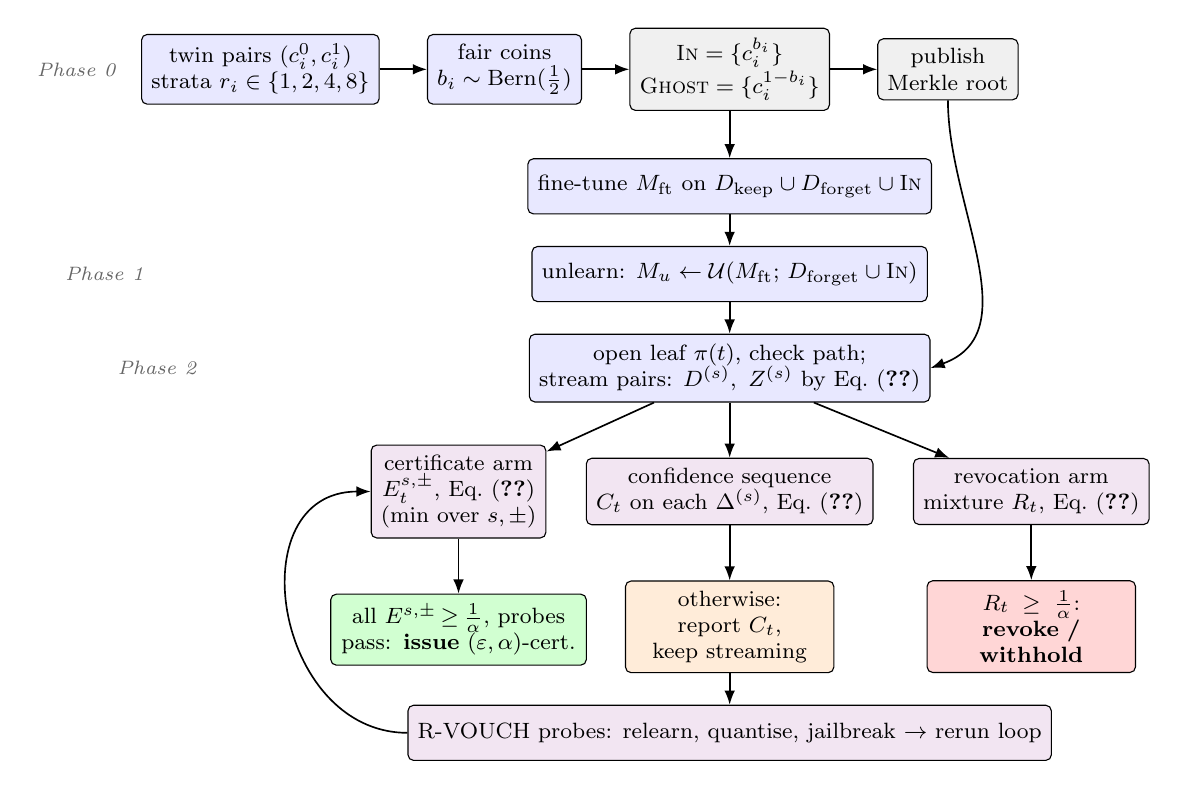
\begin{tikzpicture}[
  font=\footnotesize,
  node distance=4mm and 6mm,
  box/.style={draw, rounded corners=2pt, align=center, inner sep=3.5pt,
              minimum height=7mm},
  data/.style={box, fill=gray!12},
  proc/.style={box, fill=blue!9},
  eng/.style={box, fill=violet!10},
  good/.style={box, fill=green!18},
  bad/.style={box, fill=red!16},
  wait/.style={box, fill=orange!15},
  arr/.style={-{Latex[length=1.8mm]}, semithick},
  lab/.style={font=\scriptsize\itshape, text=black!60}
]
% Phase 0 row
\node[proc] (gen) {twin pairs $(c_i^0,c_i^1)$\\ strata $r_i\in\{1,2,4,8\}$};
\node[proc, right=of gen] (coin) {fair coins\\ $b_i\sim\Bern(\frac12)$};
\node[data, right=of coin] (split) {$\textsc{In}=\{c_i^{b_i}\}$\\
  $\textsc{Ghost}=\{c_i^{1-b_i}\}$};
\node[data, right=of split] (commit) {publish\\ Merkle root};
\node[proc, below=6mm of split] (ft) {fine-tune $M_{\mathrm{ft}}$ on
  $D_{\text{keep}}\cup D_{\text{forget}}\cup \textsc{In}$};
\node[proc, below=of ft] (unlearn) {unlearn: $M_u \gets \Ucal(M_{\mathrm{ft}};\,
  D_{\text{forget}}\cup\textsc{In})$};
\node[proc, below=of unlearn] (score) {open leaf $\pi(t)$, check path;\\
  stream pairs: $D^{(s)},\ Z^{(s)}$ by Eq.~\eqref{eq:sign}};
% three coupled processes
\node[eng, below=7mm of score] (cs) {confidence sequence\\
  $C_t$ on each $\Delta^{(s)}$, Eq.~\eqref{eq:cs}};
\node[eng, left=5mm of cs] (cert) {certificate arm\\
  $E_t^{s,\pm}$, Eq.~\eqref{eq:wealthwor}\\ (min over $s,\pm$)};
\node[eng, right=5mm of cs] (rev) {revocation arm\\
  mixture $R_t$, Eq.~\eqref{eq:revmix}};
% decisions
\node[good, below=7mm of cert, text width=30mm] (issue)
  {all $E^{s,\pm}\!\ge\!\frac1\alpha$, probes pass: \textbf{issue}
   $(\eps,\alpha)$-cert.};
\node[bad, below=7mm of rev, text width=24mm] (revoke) {$R_t \ge \frac1\alpha$:\\
  \textbf{revoke / withhold}};
\node[wait, below=7mm of cs, text width=24mm] (undet) {otherwise: report $C_t$,
  keep streaming};
\node[eng, below=4mm of undet] (probes) {R-VOUCH probes: relearn, quantise,
  jailbreak $\to$ rerun loop};
% arrows
\draw[arr] (gen) -- (coin);
\draw[arr] (coin) -- (split);
\draw[arr] (split) -- (commit);
\draw[arr] (split) -- (ft);
\draw[arr] (ft) -- (unlearn);
\draw[arr] (unlearn) -- (score);
\draw[arr] (commit.south) to[out=-90, in=20] (score.east);
\draw[arr] (score) -- (cert);
\draw[arr] (score) -- (cs);
\draw[arr] (score) -- (rev);
\draw[arr] (cert) -- (issue);
\draw[arr] (rev) -- (revoke);
\draw[arr] (cs) -- (undet);
\draw[arr] (undet) -- (probes);
\draw[arr] (probes.west) to[out=180, in=180, looseness=1.4] (cert.west);
% phase labels
\node[lab, left=2mm of gen.west, anchor=east] {Phase 0};
\node[lab, left=48mm of unlearn.west, anchor=east] {Phase 1};
\node[lab, left=41mm of score.west, anchor=east] {Phase 2};
\end{tikzpicture}}
\caption{The VOUCH pipeline. Phase 0 plants paired ghost canaries and commits to the
manifest as a Merkle tree; Phase 1 unlearns with the in-twins riding along; Phase 2
opens one leaf at a time in a committed random order and streams the pairs through
three coupled anytime-valid processes---the per-score certificate minimum, the betting
confidence sequence, and the revocation mixture---whose boundary crossings trigger
issuance, continued monitoring, or revocation. R-VOUCH probes rerun the loop on
relearned, quantised, and jailbroken variants before a robust certificate is issued.}
\label{fig:flowchart}
\end{figure}

\section{Theory}\label{sec:theory}
Our guarantees rest on one structural fact---the null we plant is exact---and on the
supermartingale property of betting. The proofs are short, and their brevity is the
point: the design does the work, so we give every proof in full. Throughout,
$\F_{t-1}$ denotes the verifier's filtration of Section~\ref{sec:filtration},
generated by everything opened through step $t-1$; all bets and mixture weights are
$\F_{t-1}$-measurable (predictable).

A word on what changed in this version, since it is the technical heart of the paper.
An earlier draft defined the certified quantity as the \emph{marginal} sign
probability $\Pr[Z_i^{(s)}=1]$ and proved coverage from a supermartingale argument
that in fact requires the stronger conditional statement
$\Efrak[Z_i^{(s)}\mid\F_{i-1}] \ge p_0$ at every step. The two coincide when signs
are independent and identically distributed across pairs, and they come apart when
they are not---which is exactly our situation, since every canary passes through one
jointly trained and unlearned model. Section~\ref{sec:exp-dependence} measures the
gap and finds it large. We therefore restate the certificate against the quantity the
protocol actually controls, and we obtain a guarantee that needs no independence,
no exchangeability across pairs, and no homogeneity across templates or repetition
strata.

\subsection{The exact null}

\begin{theorem}[Exact conditional null]\label{thm:null}
Suppose the unlearned model $M_u$ is conditionally independent of the coin vector
$b=(b_1,\dots,b_m)$ given the pair contents $C=\{(c_i^0,c_i^1)\}$; exact unlearning
and retraining-from-scratch both satisfy this. Then for every score $s\in\F$, every
step $t$, and the pair $j=\pi(t)$ opened at that step,
\[
Z_j^{(s)} \mid \F_{t-1} \;\sim\; \Bern(\tfrac12) \quad\text{exactly,}
\]
for any model, any score, and any set of query prompts. In particular the sign
sequence is a sequence of exact conditional fair coins \emph{whether or not the signs
are independent across pairs}.
\end{theorem}

\begin{proof}
Enlarge $\F_{t-1}$ to $\G_{t-1} = \F_{t-1} \vee \sigma\bigl(\pi(t),\,
\{c_j^0, c_j^1\}\bigr)$, which reveals the position and the \emph{unordered} pair
opened at step $t$ but not its coin; this is legitimate because the manifest is
committed leaf-by-leaf (Section~\ref{sec:filtration}), so $b_j$ is opened only at
step $t$. Given $\G_{t-1}$ the two numbers $s(M_u, x)$ and $s(M_u, y)$ attached to
the unordered pair $\{x,y\}=\{c_j^0,c_j^1\}$ are determined. The coin $b_j$ is
independent of the other coins and of $C$ by construction, and independent of $M_u$
given $C$ by hypothesis; nothing opened before step $t$ involves $b_j$. Hence
$b_j \mid \G_{t-1} \sim \Bern(\tfrac12)$. Since $b_j$ decides which of the two
determined numbers is the in-twin's,
\[
D_j^{(s)} \;=\; s(M_u, c_j^{\text{in}}) - s(M_u, c_j^{\text{ghost}})
\;=\; \pm\bigl|s(M_u,x) - s(M_u,y)\bigr|
\]
with the two signs equally likely, so $D_j^{(s)} \overset{d}{=} -D_j^{(s)}$ given
$\G_{t-1}$. Therefore $\Pr[D_j^{(s)}>0\mid\G_{t-1}] = \Pr[D_j^{(s)}<0\mid\G_{t-1}]$,
and the committed tie-break coin splits any atom at zero equally, giving
$Z_j^{(s)}\mid\G_{t-1}\sim\Bern(\tfrac12)$. Averaging over $\G_{t-1}\supseteq\F_{t-1}$
gives the claim. No property of the model, the score, the query set, or the
dependence between pairs was used beyond measurability.
\end{proof}

Theorem~\ref{thm:null} is the reason VOUCH needs neither shadow models nor a
retrained reference: the null distribution is not estimated or assumed but generated
by our own coins, and it is exact at finite $m$. It is worth being explicit about why
the dependence objection does not bite here. The signs $Z_1^{(s)},\dots,Z_m^{(s)}$
are indeed dependent---they share one model---but the proof never asks for
independence. It asks only that the coin governing the pair opened at step $t$ still
be fair given everything opened before, and under exact unlearning it is, because the
model carries no information about it. The revocation arm therefore inherits an exact
null with no further conditions. The certificate arm, whose null is the composite
``some score still leaks,'' is where dependence has to be confronted, and that is the
next subsection.

\subsection{The certified quantity and the certificate}\label{sec:certquantity}

Once $M_u$ and the manifest exist, the sign vector $z^{(s)} = (z_1^{(s)},\dots,
z_m^{(s)})$ of the committed cohort is fixed; the only randomness left to the audit
is the reveal order and the tie coins. We therefore certify the advantage the
declared score actually achieves against that cohort.

\begin{definition}[Realised cohort advantage]\label{def:delta}
For $s\in\F$ the \emph{realised cohort advantage} is
\begin{equation}\label{eq:delta}
\Delta^{(s)} \;=\; \frac{2}{m}\sum_{i=1}^{m} z_i^{(s)} \;-\; 1
\;=\; 2\,\Pr\nolimits_{I}\bigl[z_I^{(s)}=1\bigr] - 1 ,
\end{equation}
the advantage of the rule ``guess that the twin scoring higher under $s$ is the
in-twin'' when the pair index $I$ is drawn uniformly from the committed cohort. Two
coarser quantities sit above it: the \emph{mechanism-level} advantage
$\Delta^{(s)}_C = \Efrak_b[\Delta^{(s)} \mid C, \xi]$, averaging over the inclusion
coins with the pair contents $C$ and the training randomness $\xi$ held fixed; and the
\emph{super-population} advantage $\bar\Delta^{(s)} = \Efrak[\Delta^{(s)}]$, averaging
over $C$ and $\xi$ as well.
\end{definition}

$\Delta^{(s)}$ is the quantity an auditor of \emph{this} model wants bounded, and it
is the one the protocol controls exactly; Definition~\ref{def:cert} is stated for it.
Proposition~\ref{prop:transfer} climbs one level, from $\Delta^{(s)}$ to
$\Delta^{(s)}_C$, at a stated cost in tolerance. We do not climb the second level to
$\bar\Delta^{(s)}$: that would need concentration over the draw of corpora, which we
neither prove nor assume. Where the experiments report a ``super-population'' verdict
they mean the fixed-boundary process of the earlier design, whose null is the
predictable conditional mean; we keep both columns throughout so that the reader can
see which claims survive at which tolerance.

\begin{definition}[$(\eps,\alpha)$-forgetting certificate]\label{def:cert}
Fix a tolerance $\eps \in (0,1)$, an error budget $\alpha \in (0,1)$, and the boundary
$p_0 = \tfrac12 + \tfrac\eps2$. An $(\eps,\alpha)$-forgetting certificate for $M_u$
over the class $\F$ is a data-dependent stopping decision that asserts
$\sup_{s\in\F}|\Delta^{(s)}| < \eps$, issued by a procedure with the guarantee that,
whenever in truth $\sup_{s\in\F}|\Delta^{(s)}| \ge \eps$, the probability that a
certificate is \emph{ever} issued---at any stopping time, under any monitoring
rule---is at most $\alpha$.
\end{definition}

The two-sidedness in Definition~\ref{def:cert} is deliberate: $\Delta^{(s)} \le -\eps$,
the over-forgetting regime in which the in-twin scores conspicuously \emph{below} its
never-seen partner, is membership leakage exactly as much as $\Delta^{(s)} \ge \eps$
is, and Section~\ref{sec:exp} shows that gradient-ascent unlearning lands there in
practice.

\begin{theorem}[Certificate coverage under arbitrary dependence]\label{thm:cert}
Reveal the cohort in a uniformly random order $\pi$ drawn by the verifier
\emph{independently of the realised sign vectors} $\{z^{(s)}\}_{s\in\F}$ and committed
before any query, and for each score $s$ and direction run the wealth process of
Eq.~\eqref{eq:wealthwor} with stakes confined to
$\lambda_t^{s,+} \in [0,\, c/(1-p_0(t)))$ and
$\lambda_t^{s,-} \in [0,\, c/\bar p_0(t))$ for some fixed $c < 1$, against the
predictable without-replacement boundary
\begin{equation}\label{eq:worboundary}
p_0(t) \;=\; \frac{m\,p_0 \;-\; \sum_{u<t} Z^{(s)}_{\pi(u)}}{m-t+1},
\end{equation}
declaring the null refuted outright if ever $p_0(t) > 1$. Issue the certificate only
when \emph{every} per-score, per-direction process exceeds $1/\alpha$. Then for any
class $\F$ and any stopping rule,
\[
\Pr\bigl[\text{a false }(\eps,\alpha)\text{-certificate is ever issued}\bigr] \le \alpha
\qquad\text{whenever } \sup_{s\in\F}|\Delta^{(s)}| \ge \eps .
\]
The guarantee is exact and finite-sample, and it holds \emph{conditionally on the
cohort's sign vectors}: no independence across pairs, no exchangeability across
pairs, and no homogeneity across templates or repetition strata is assumed. No
multiplicity correction over $\F$ is required. The one thing that \emph{is} assumed
is the independence of $\pi$ from the signs, and Remark~\ref{rem:order} explains why
it is not free.
\end{theorem}

\begin{proof}
Suppose the certification claim is false, so some score $s^\ast$ and direction violate
the tolerance; say $\Delta^{(s^\ast)} \ge \eps$, i.e.\ the cohort mean
$\mu = \tfrac1m\sum_i z_i^{(s^\ast)}$ satisfies $\mu \ge p_0$ (the case
$\Delta^{(s^\ast)} \le -\eps$ is symmetric, run against $1-p_0$). Condition on the
entire sign vector $z^{(s^\ast)}$; the remaining randomness is the uniform
permutation $\pi$, and sequential reveal of a uniform permutation is precisely simple
random sampling without replacement. Hence the conditional mean of the next sign is
the mean of the unrevealed remainder,
\[
\Efrak\bigl[Z^{(s^\ast)}_{\pi(t)} \,\big|\, \F_{t-1}\bigr]
= \frac{m\mu - \sum_{u<t} Z^{(s^\ast)}_{\pi(u)}}{m-t+1}
\;\ge\; \frac{m p_0 - \sum_{u<t} Z^{(s^\ast)}_{\pi(u)}}{m-t+1}
\;=\; p_0(t),
\]
using $\mu \ge p_0$. Each wealth factor therefore has conditional mean
\[
\Efrak\bigl[\,1 + \lambda_t\,(p_0(t) - Z^{(s^\ast)}_{\pi(t)}) \,\big|\, \F_{t-1}\bigr]
= 1 + \lambda_t\bigl(p_0(t) - \Efrak[Z^{(s^\ast)}_{\pi(t)} \mid \F_{t-1}]\bigr) \;\le\; 1,
\]
since $\lambda_t \ge 0$ is predictable. Nonnegativity is the other half and needs the
stake restriction: with $Z \in \{0,1\}$ the factor $1 + \lambda_t(p_0(t) - Z)$ is
minimised at $Z = 1$, where it equals $1 - \lambda_t(1 - p_0(t)) \ge 1 - c > 0$ by
$\lambda_t < c/(1-p_0(t))$; the mirror arm is identical with $\bar p_0(t)$ in place of
$1 - p_0(t)$. (This bound is why the implementation must derive the stake cap from the
\emph{same} clamped boundary the payoff is evaluated at; see
Appendix~\ref{app:repro}.) So the process is a nonnegative supermartingale started at
one, and Ville's inequality gives
$\Pr[\exists t: E_t^{s^\ast,+} \ge 1/\alpha] \le \alpha$. The refutation branch is
never taken under the null, because $p_0(t) \le \Efrak[Z_{\pi(t)}\mid\F_{t-1}] \le 1$.
Issuing the certificate requires \emph{every} process to exceed $1/\alpha$---in
particular the violating score's own---so a false certificate is issued with
conditional probability at most $\alpha$, uniformly over stopping rules; averaging
over the sign vectors preserves the bound. No union bound over $\F$ is needed because
the argument runs entirely through the single process attached to the violating
score.
\end{proof}

Two consequences are worth naming because they shape how the certificate should be
read. First, the guarantee spends no assumption on the \emph{data}: whatever
dependence the shared model induces among the signs, it is absorbed by conditioning on
the realised sign vector, and the only randomness the proof spends is the verifier's
own permutation. Second, and less comfortably, a cohort audited to exhaustion resolves
\emph{deterministically}: at $t=m$ the realised mean is known, and no inference
remains. The betting machinery therefore buys three things---early stopping at a
fraction of the query budget, validity under continuous monitoring and across
deletion waves, and the alarm arm, whose null is the genuinely stochastic one of
Theorem~\ref{thm:null}---rather than buying the cohort statement itself. We think
this is the honest way to describe what a canary audit can do, and
Section~\ref{sec:exp-baselines} quantifies each of the three.

\begin{remark}[The reveal order must be the verifier's own randomness]\label{rem:order}
Theorem~\ref{thm:cert} conditions on the sign vector and spends the permutation, so it
needs $\pi \perp \{z^{(s)}\}$. That is not a formality here. A provider
who can locate the cohort---and Section~\ref{sec:exp-detect} shows that is
cheap---could, if it also knew $\pi$, arrange which pairs are revealed early. The
released implementation therefore draws $\pi$ from one of three sources, and records
which on the certificate. A \emph{public randomness beacon} is the recommended one:
the verifier fetches a drand round published \emph{after} the manifest commitment and
seeds $\pi$ with $H(\text{root} \,\|\, \text{beacon randomness})$, so the order is
unpredictable to the provider before the round exists, independent of the signs, and
reconstructible afterwards by anyone holding the certificate---the audit's own
randomness becomes as checkable as its commitment. Failing network access, the
verifier draws from operating-system entropy, which satisfies the hypothesis but is
not third-party verifiable. The third source is the run seed, which is what produced
the results in this paper and which does \emph{not} satisfy the hypothesis, since that
seed also seeds cohort generation and training; nothing in the pipeline exploits the
coupling, but the condition is not met, and Appendix~\ref{app:repro} records exactly
where. Binding the beacon value to the commitment matters in both directions: drawing
the beacon first would let a provider grind the manifest against a known order.
\end{remark}

\begin{proposition}[Transfer to the coin-averaged advantage]\label{prop:transfer}
Fix the pair contents $C$ and the training randomness $\xi$, and write
$\Delta^{(s)}_C = \Efrak_b\bigl[\Delta^{(s)} \,\big|\, C, \xi\bigr]$ for the
advantage averaged over the inclusion coins alone---the advantage the unlearning
\emph{mechanism} yields on this corpus. Assume \emph{bounded coin influence}:
flipping a single coin $b_i$ changes at most $\kappa$ of the $m$ signs
$z_j^{(s)}$. Then for any $\alpha' \in (0,1)$, with probability at least
$1-\alpha'$,
\begin{equation}\label{eq:transfer}
\bigl|\Delta^{(s)} - \Delta^{(s)}_C\bigr| \;\le\;
\kappa\,\sqrt{\frac{2\log(2/\alpha')}{m}} .
\end{equation}
Consequently a cohort certificate at tolerance $\eps$ implies a mechanism-level
certificate at tolerance $\eps + \kappa\sqrt{2\log(2/\alpha')/m}$, at total error
level $\alpha + \alpha'$.
\end{proposition}

\begin{proof}
Write $f(b) = \tfrac2m\sum_j z_j^{(s)} - 1$ as a function of the coin vector, the
other randomness held fixed. Changing one coordinate changes $\sum_j z_j^{(s)}$ by at
most $\kappa$ by hypothesis, so $f$ has bounded differences $c_i = 2\kappa/m$.
McDiarmid's inequality gives
$\Pr[|f - \Efrak_b f| \ge u] \le 2\exp(-2u^2/\sum_i c_i^2) = 2\exp(-u^2 m/(2\kappa^2))$,
with the expectation over the coins and $(C,\xi)$ held fixed---which is exactly
$\Delta^{(s)}_C$; setting the right-hand side to $\alpha'$ yields
\eqref{eq:transfer}.
\end{proof}

Three qualifications travel with Proposition~\ref{prop:transfer} and we would rather
state them than let a reader over-read the bound. First, it bounds the distance to
$\Delta^{(s)}_C$, the \emph{coin-averaged} advantage on this corpus, not to
$\bar\Delta^{(s)} = \Efrak[\Delta^{(s)}]$ of Definition~\ref{def:delta}, which
additionally averages over the draw of $C$ and $\xi$; closing that second gap requires
a further concentration step over corpora that we do not have and do not claim.
Second, the bound is informative only when $\kappa = o(\sqrt m)$: at
$\kappa = \Theta(m)$ it is vacuous. Under exact unlearning $\kappa = 1$ holds
trivially, since a coin that leaves no trace in the model can only affect its own
pair's sign; away from it, an influential coin can move the model and hence many
signs, which is precisely the regime where the transfer is wanted. Third, the size of
the price is worth internalising: at $m=512$, $\alpha'=0.05$ and $\kappa=1$ the
inflation is $0.12$, which is why a mechanism-level claim at $\eps = 0.05$ needs a
cohort an order of magnitude larger than a cohort claim at the same tolerance---a gap
Section~\ref{sec:exp-bench} reports rather than elides.

\begin{remark}[Why the intuitive mixture fails]\label{rem:mixture}
It is tempting to run a \emph{single} certificate process on the adaptively reweighted
sign $\bar Z_t = \sum_s w_s Z_t^{(s)}$, and indeed this is valid for the revocation arm,
whose null makes every component an exact conditional fair coin. It is \emph{not}
valid for the certificate, whose composite null is ``some score still leaks.'' The
failure is easy to exhibit: take $\Delta^{(s_1)} = \eps$ exactly at the boundary and
$\Delta^{(s_2)} = \dots = 0$ clean. Then
$\Efrak[\bar Z_t \mid \F_{t-1}] = w_1 p_0 + (1 - w_1)/2 < p_0$ whenever $w_1 < 1$, so
each factor of the mixture's certificate process has conditional mean strictly greater
than one: the process is a \emph{sub}martingale under the null and crosses $1/\alpha$
with probability approaching one. Worse, the violation is generic rather than
adversarial, because discrimination-driven reweighting moves weight \emph{away} from
the one leaking score under partial unlearning. Against this construction---which is
our own earlier design, not a published method---we measured a false-certification
rate of $0.996$ against $0.007$ for the per-score minimum
(Table~\ref{tab:soundness}), which is why VOUCH requires consensus rather than an
average.
\end{remark}

\subsection{Power, confidence sequences, and composition}

\begin{theorem}[Power, fixed-boundary process]\label{thm:power}
Consider the \emph{super-population} arm, i.e.\ the process of
Eq.~\eqref{eq:wealthwor} run against the fixed boundary $p_0(t) \equiv p_0$ with signs
i.i.d.\ across pairs. If $|\Delta^{(s)}| < \eps$ for all $s$ and the bets have
sublinear regret (the mixture of Section~\ref{sec:engine} qualifies), then
$\tfrac1t \log E_t \to \KL(\Bern(p)\,\|\,\Bern(p_0))$ almost surely for each process,
and the expected certification time is
$\Efrak[\tau^*] = (1+o(1))\,\log(1/\alpha)/\min_{s,\pm}\KL$, the expectation being
taken under exact unlearning and the asymptotics in small $\eps$. Since
\begin{equation}\label{eq:klexp}
\KL\bigl(\Bern(\tfrac12)\,\big\|\,\Bern(\tfrac12 + \tfrac\eps2)\bigr)
\;=\; -\tfrac12\log\bigl(1-\eps^2\bigr)
\;=\; \tfrac{\eps^2}{2} + O(\eps^4),
\end{equation}
this is approximately $2\log(1/\alpha)/\eps^2$ pairs.
\end{theorem}

The restriction to the fixed boundary is not cosmetic. Under without-replacement reveal the log-wealth increments are
neither independent nor identically distributed, the boundary $p_0(t)$ moves, and the
admissible stake range moves with it---so ``the best constant bet'' is not well
defined, and neither the $O(\log t)$ ONS regret bound (which assumes a fixed convex
domain) nor the Krichevsky--Trofimov redundancy bound (which assumes a fixed $p_0$)
transfers as stated. Theorem~\ref{thm:power} should therefore be read as sizing the
cohort for a \emph{mechanism-level} claim. For the finite-cohort target we do not have
a matching analysis; its certification time is capped by $m$, since the claim resolves
deterministically once the cohort is exhausted, and we report its behaviour
empirically instead (Table~\ref{tab:power}, cohort column).

\begin{proof}
Fix one process, say the upper process for a score with true sign probability
$p < p_0$. For a constant bet $\lambda$, the log-wealth increments
$\log(1 + \lambda(p_0 - Z_t))$ are i.i.d.\ with mean
$f(\lambda) = p \log(1 - \lambda(1 - p_0)) + (1-p)\log(1 + \lambda p_0)$, so by the
strong law $\tfrac1t \log E_t \to f(\lambda)$ almost surely. The Kelly-optimal
constant bet is $\lambda^\ast = (p_0 - p)/(p_0(1 - p_0))$: substituting it turns the
two possible wealth factors into the Bernoulli likelihood ratios
$1 - \lambda^\ast(1 - p_0) = p/p_0$ and $1 + \lambda^\ast p_0 = (1-p)/(1-p_0)$,
so $f(\lambda^\ast) = p \log\tfrac{p}{p_0} + (1-p)\log\tfrac{1-p}{1-p_0}
= \KL(\Bern(p)\,\|\,\Bern(p_0))$, and no constant bet can do better because $f$ is
concave with this maximum. A betting strategy whose log-wealth regret against the best
constant bet is $o(t)$ therefore attains the same limit; the ONS expert has $O(\log t)$
regret, the KT plug-in \eqref{eq:kt} achieves $\KL - \tfrac{1}{2t}\log t$ directly by
the Krichevsky--Trofimov redundancy bound, and the uniform mixture over eight experts
trails its best expert by at most the constant $\log 8$, so all three satisfy the
hypothesis. For the crossing time, the process rejects when
$\log E_t \ge \log(1/\alpha)$; since $\tfrac1t\log E_t \to \KL$ almost surely, the
first-crossing time $\tau^\ast$ satisfies
$\Efrak[\tau^\ast] = (1 + o(1)) \log(1/\alpha)/\KL$ by the standard Wald argument, and
issuance waits for the \emph{slowest} process, whose drift is $\min_{s,\pm} \KL$.
Finally, under exact unlearning $p = \tfrac12$ for every score, and
\[
\KL\bigl(\Bern(\tfrac12)\,\big\|\,\Bern(p_0)\bigr)
= \tfrac12\log\tfrac{1/2}{p_0} + \tfrac12\log\tfrac{1/2}{1-p_0}
= -\tfrac12\log\bigl(4p_0(1-p_0)\bigr)
= -\tfrac12\log(1-\eps^2),
\]
whose expansion is \eqref{eq:klexp}, giving
$\Efrak[\tau^\ast] \approx 2\log(1/\alpha)/\eps^2$.
\end{proof}

Theorem~\ref{thm:power} tells the provider how large a canary cohort to plant. An
$\eps = 0.1$ certificate at $\alpha = 0.05$ needs on the order of $600$ pairs, an
$\eps = 0.05$ certificate roughly $2{,}400$, and an $\eps=0.02$ certificate roughly
$15{,}000$; because the drift equals the Kullback--Leibler divergence---the
information-theoretic optimum for testing $\Bern(\tfrac12)$ against $\Bern(p_0)$---no
valid procedure can do better by more than a constant factor. We note that an earlier
version of this theorem reported the expansion as $\eps^2/8$ and the sample size as
$8\log(1/\alpha)/\eps^2$; \eqref{eq:klexp} corrects it. The numerical columns of
Table~\ref{tab:power} were computed from the exact divergence and are unaffected.

\begin{theorem}[Finite-cohort certification time]\label{thm:cohortpower}
Fix a score $s$ and run the upper certificate process of
Theorem~\ref{thm:cert}: the without-replacement boundary
\eqref{eq:worboundary} with the rule that the null is refuted outright once
$p_0(t) > 1$. Let the committed cohort of size $m$ carry exactly $j$ signs
$z_i^{(s)} = 1$, and let $k_0 = \lceil m p_0 \rceil$ be the least number of
such signs compatible with the null $\Delta^{(s)} \ge \eps$. If
$j \le k_0 - 2$---the realised cohort sits at least two pairs below the
boundary---then the process refutes, and hence certifies at \emph{any}
$\alpha$, by the stopping time
\begin{equation}\label{eq:cohortworst}
\tau^\ast \;\le\; m - (k_0 - j) + 2
\qquad\text{for \emph{every} reveal order } \pi,
\end{equation}
and, under the uniformly random $\pi$ that Theorem~\ref{thm:cert} requires,
\begin{equation}\label{eq:cohortmean}
\Efrak[\tau^\ast] \;\le\; \frac{(m - k_0 + 1)(m+1)}{m - j + 1} \;+\; 1 ,
\end{equation}
with equality when the decision is reached by refutation. The lower arm is
the mirror statement with $z$ replaced by $1-z$ and $p_0$ by $1-p_0$; the
two-sided certificate over a class $\F$ is issued by the largest of the
$2|\F|$ individual bounds. Neither bound involves $\alpha$, the betting
strategy, or $|\F|$.
\end{theorem}

\begin{proof}
Refutation fires at the first $t$ with $p_0(t) > 1$, i.e.\ with
$m p_0 - \sum_{u<t} Z_{\pi(u)} > m - t + 1$. Writing $S_{t-1}$ for the
revealed count of ones and $W_{t-1} = (t-1) - S_{t-1}$ for the revealed
count of zeros, and using $S_{t-1} + (m - t + 1) = m - W_{t-1}$, the
condition is $m - W_{t-1} < m p_0$, that is $W_{t-1} > m(1 - p_0)$. Both
sides being compared to an integer, this is exactly
$W_{t-1} \ge m - k_0 + 1 =: r$, whether or not $m p_0$ is an integer.
Refutation therefore occurs one step after the $r$-th zero is revealed:
$\tau^\ast = 1 + \pi\text{-position of the } r\text{-th zero}$. The cohort
contains $m - j$ zeros, and $r \le m - j - 1$ exactly when $j \le k_0 - 2$,
so under that hypothesis the $r$-th zero is revealed at some position
$\le m - 1$ and $\tau^\ast \le m$.

For \eqref{eq:cohortworst}, the position of the $r$-th zero is largest when
every one precedes every zero, putting it at $j + r = j + m - k_0 + 1$;
adding the one step gives the bound, and the ordering that attains it shows
it is tight. For \eqref{eq:cohortmean}, let $M = m - j$ be the number of
zeros. In a uniformly random arrangement the $M$ zeros split the $m - M$
ones into $M+1$ exchangeable gaps, so the expected number of ones preceding
the $r$-th zero is $r(m - M)/(M + 1)$ and the expected position of that zero
is $r + r(m-M)/(M+1) = r(m+1)/(M+1)$. Adding one step gives
\eqref{eq:cohortmean}.

Finally, the argument never inspects the stake $\lambda_t$: refutation is a
statement about which cohort compositions remain feasible, so it holds for
every predictable betting strategy, and the certificate's actual stopping
time is the minimum of this time and the time its wealth crosses $1/\alpha$
by ordinary growth.
\end{proof}

Theorem~\ref{thm:cohortpower} is the finite-population counterpart that
Theorem~\ref{thm:power} could not supply. Under without-replacement reveal
the log-wealth increments are neither independent nor identically
distributed and the regret bounds behind Theorem~\ref{thm:power} do not
transfer, so we bound the cohort target's stopping time by a different
route: not by how fast wealth grows, but by when the null's remaining
feasible compositions run out. The two mechanisms run in parallel and the
process stops at whichever fires first, which is what makes the cohort
column of Table~\ref{tab:power} legitimately faster than the
Kullback--Leibler column rather than mysteriously so. Their regimes are
also easy to tell apart: exponential growth dominates when the cohort is
large relative to $\log(1/\alpha)/\KL$, and the feasibility bound binds when
it is not, which is exactly the tight-tolerance regime of
Section~\ref{sec:exp-tight}. At $m = 384$, $\eps = 0.2$ and a cohort at
chance ($j = m/2$), \eqref{eq:cohortmean} gives $308$ pairs against a
measured median of $165$: the wealth process usually wins, and the
feasibility bound is the guarantee that holds when it does not.

\begin{remark}[Per-score versus simultaneous confidence sequences]\label{rem:cs}
Each score's confidence sequence \eqref{eq:cs} covers that score's own advantage
$\Delta^{(s)}$ with uniform-in-time probability $1-\alpha$; the guarantee is
\emph{per score}. Two derived statements should be distinguished. The reported
$\max_{s\in\F} U_t^{(s)}$ \emph{is} a valid level-$\alpha$ anytime upper bound on
$\sup_{s\in\F}\Delta^{(s)}$ with no multiplicity correction, because the maximising
index of the population quantities is a fixed, non-random index once the cohort is
fixed, and that single score's own sequence is the only one the argument needs.
Simultaneous two-sided coverage of \emph{all} $|\F|$ advantages, on the other hand,
costs a union bound and holds at level $|\F|\alpha$; we report intervals at that
corrected level wherever we display the whole class.
\end{remark}

\begin{theorem}[Streaming composition, in both directions]\label{thm:streaming}
Let deletion waves $k = 1,\dots,K$ use cohorts with independent coins.
\emph{(a) Certificates compose by consensus.} Claiming that the whole history is clean
only when every wave has individually earned its certificate keeps the probability of a
false history-wide claim at or below $\alpha$ for any $K$; multiplying certificate
e-values instead tests the intersection null ``every wave is bad,'' whose rejection
certifies merely that \emph{some} wave is clean.
\emph{(b) Alarms compose by product.} Under the intersection null ``every wave was
exactly unlearned'' each per-wave revocation process is a supermartingale, so their
product is one too and crosses $1/\alpha$ with probability at most $\alpha$; the product
accumulates leakage spread so thinly across waves that no single wave reveals it.
\emph{(c)} Per-wave alarms with $\alpha$-spending $\alpha_k = \alpha 2^{-(k+1)}$ control
family-wise false revocation over an unbounded history.
\end{theorem}

\begin{proof}
\emph{(a)} Suppose the history-wide claim is false, so some wave $k^\ast$ truly has
$\sup_s |\Delta^{(s),(k^\ast)}| \ge \eps$. The all-pass rule claims only when every
wave has individually issued, so claiming requires wave $k^\ast$'s own per-score
minimum process to cross $1/\alpha$, an event of probability at most $\alpha$ by
Theorem~\ref{thm:cert}---independently of $K$ and of how the auditor schedules the
waves. For the negative half of the statement, note that a product
$\prod_k E^{(k)}$ of \emph{certificate} e-values is, by construction, an e-value for
the intersection null $\bigcap_k \{\text{wave } k \text{ bad}\}$; rejecting an
intersection establishes only the disjunction ``some wave is clean.'' In the
one-bad-wave scenario the clean waves' e-values grow without bound and drag the
product over $1/\alpha$ regardless of the bad wave. We measure the damage rather than
assert it: over $500$ ten-wave histories containing one genuinely bad wave, the
product rule issues a false history-wide certificate in \emph{every} history whose bad
wave truly violates the tolerance, against $0.000$ for the all-pass rule
(Table~\ref{tab:certprod}).

\emph{(b)} Under the intersection null, Theorem~\ref{thm:null} applies wave by wave,
so each $R^{(k)}$ is a nonnegative supermartingale with initial value one with respect
to the combined filtration, and cohorts across waves are independent by construction.
Conditional on $\F_{t-1}$, the increment of the product
$\prod_k R^{(k)}$ at any arrival is the increment of the single wave whose pair is
revealed, which has conditional mean at most one; the product is therefore itself a
nonnegative supermartingale started at one, for any adapted within-wave sampling times,
and Ville's inequality bounds its crossing probability by $\alpha$. Its power against
distributed leakage is additive in the exponent: if every wave carries advantage
$\Delta_0 > 0$, each factor drifts upward at rate
$\KL(\Bern(\tfrac12 + \tfrac{\Delta_0}2) \,\|\, \Bern(\tfrac12))$ per pair, so the
product crosses after roughly $\log(1/\alpha)/(m \cdot \KL)$ waves even when no single
wave is individually detectable.

\emph{(c)} Give wave $k$ its own alarm at level $\alpha_k = \alpha 2^{-(k+1)}$. By
Ville applied per wave, the probability that a truly clean wave $k$ ever alarms is at
most $\alpha_k$, and the union bound over an unbounded horizon costs
$\sum_{k \ge 1} \alpha 2^{-(k+1)} \le \alpha/2 \le \alpha$.
\end{proof}

\begin{proposition}[A magnitude-aware alarm]\label{prop:magnitude}
Under the null of Theorem~\ref{thm:null}, $\mathrm{sign}(D_t)$ is a fair coin even
conditional on $|D_t|$, so wealth factors of the form
$1 + \lambda_t\,\mathrm{sign}(D_t)\,g_t$ are an exact e-process for any predictable
stake $g_t \in [0,1]$ measurable with respect to the past and $|D_t|$. Taking $g_t$ to
be the predictable rank of $|D_t|$ concentrates bets on the large-effect pairs where
sparse memorisation lives, and halves detection time under $5\%$-sparse leakage
(Section~\ref{sec:exp-ablation}). Because it bets aggressively we report it as an
optional power enhancement and keep the sign-based arm as the default.
\end{proposition}

\begin{proof}
Symmetry of the conditional law of $D_t$ (Theorem~\ref{thm:null}) means that
conditioning on the magnitude $|D_t|$ leaves the sign exactly fair:
$\Efrak[\mathrm{sign}(D_t) \mid |D_t|, \F_{t-1}] = 0$, with ties randomised by the
committed coin. For any stake $g_t \in [0,1]$ that is measurable with respect to
$\F_{t-1} \vee \sigma(|D_t|)$---the predictable rank of $|D_t|$ among past magnitudes
qualifies---the tower property gives
$\Efrak[\mathrm{sign}(D_t)\, g_t \mid \F_{t-1}] = \Efrak[\,g_t\,
\Efrak[\mathrm{sign}(D_t) \mid |D_t|, \F_{t-1}] \mid \F_{t-1}] = 0$, so each factor
$1 + \lambda_t\, \mathrm{sign}(D_t)\, g_t$ with predictable $\lambda_t \in [0,1)$ has
conditional mean exactly one and stays positive. The product is a nonnegative
martingale with initial value one, hence an exact e-process, and Ville's inequality
applies as before. The power claim is empirical and quantified in
Section~\ref{sec:exp-ablation}.
\end{proof}

\begin{proposition}[One-directional bridge from certified unlearning]\label{prop:bridge}
If $\Ucal$ is $(\eps_u,\delta_u)$-certified, then
$|\bar\Delta^{(s)}| \le \tfrac{e^{\eps_u}-1}{e^{\eps_u}+1} + \delta_u$ for every $s$, so for
$\eps$ above this value VOUCH issues with probability $1 - \alpha - o(1)$. A certified
algorithm therefore passes VOUCH, as consistency demands, while VOUCH remains meaningful
at scales where $(\eps_u,\delta_u)$ certificates are unattainable.
\end{proposition}

\begin{proof}
The sign $Z^{(s)}$ is a randomised post-processing of the pipeline output: it is
computed from $M_u$ and the pair alone. $(\eps_u,\delta_u)$-certified unlearning makes
the law of $M_u$, under either value of the coin,
$(\eps_u,\delta_u)$-indistinguishable from the law of the retrained reference, under
which $Z^{(s)}$ is an exact fair coin by Theorem~\ref{thm:null}. Now view the rule
``guess that the twin with the larger score is the in-twin'' as a hypothesis test for
the coin $b_i$; its advantage is exactly
$\Pr[\text{correct}] - \Pr[\text{wrong}] = \bar\Delta^{(s)}$. The
trade-off region of \citet{kairouz2015composition} states that any test between two
$(\eps_u,\delta_u)$-indistinguishable distributions has type-I and type-II errors
satisfying $e^{\eps_u}\beta_1 + \beta_2 \ge 1 - \delta_u$ and
$\beta_1 + e^{\eps_u}\beta_2 \ge 1 - \delta_u$; adding the two constraints,
$\beta_1 + \beta_2 \ge 2(1 - \delta_u)/(1 + e^{\eps_u})$, so the advantage obeys
\[
|\bar\Delta^{(s)}| \;\le\; 1 - (\beta_1 + \beta_2)
\;\le\; 1 - \frac{2(1 - \delta_u)}{1 + e^{\eps_u}}
\;=\; \frac{e^{\eps_u} - 1}{e^{\eps_u} + 1} + \frac{2\delta_u}{1 + e^{\eps_u}}
\;\le\; \frac{e^{\eps_u} - 1}{e^{\eps_u} + 1} + \delta_u.
\]
When $\eps$ strictly exceeds this bound, every certificate process has strictly
positive drift by Theorem~\ref{thm:power} and crosses $1/\alpha$ with probability
tending to one as $m \to \infty$, while the revocation arm false-alarms with
probability at most $\alpha$; the issuance probability is therefore at least
$1 - \alpha - o(1)$.
\end{proof}

\begin{remark}[The bridge runs one way only]\label{rem:onedirection}
Proposition~\ref{prop:bridge} states that certified unlearning implies passing VOUCH.
The converse is false and we claim nothing like it: passing VOUCH does \emph{not}
imply any $(\eps_u,\delta_u)$ guarantee, does not bound the influence of any datum
outside the canary cohort, and does not constrain scores outside $\F$. The
proposition is a consistency check on the definition---an algorithm with a
parameter-space guarantee should not be flagged by a behavioural audit---and it
should not be read as a semantic equivalence in either direction.
\end{remark}

\paragraph{Scope, stated precisely.} A VOUCH certificate concerns the advantage
extractable through the declared class $\F$, on the committed canary cohort, against
the deployed model, under the honest-but-verifiable threat model of
Section~\ref{sec:setting}. It does not assert erasure in parameter space, which no
behavioural method can; it is a per-cohort statement, not a per-deletion-request one,
because per-request certificates would require per-user canaries; the transfer to the
super-population advantage costs the explicit inflation of
Proposition~\ref{prop:transfer}; and the extrapolation from planted canaries to
organic records is \emph{calibrated} through the dose--response strata and the
head-to-head comparisons of Section~\ref{sec:exp-descriptive} rather than proven. We
regard stating these limits precisely as part of the contribution, since a certificate
whose scope is overclaimed is worse than none.


\section{Experiments}\label{sec:exp}
We organise the study into three tiers so that each claim is tested where it can be
tested most sharply. The \emph{simulation tier} draws pair signs directly from their
generating distribution---exactly the object Theorems~\ref{thm:null} and
\ref{thm:cert} control---which lets us calibrate validity and power over thousands of
seeds without confounding them with the vagaries of a particular model. The
\emph{end-to-end tier} fine-tunes real models on corpora with injected canaries,
unlearns them with each subject method, and certifies the result, so that the abstract
null meets an actual training pipeline. The \emph{benchmark tier} repeats the
end-to-end protocol on the field's standard testbeds, TOFU and MUSE-News, across three
architectures.

Unless noted we use $\alpha = 0.05$, two-sided certification, the sign-based
revocation arm, the finite-cohort certificate target, LoRA fine-tuning of rank $16$,
$Q = 2$ query wrappers, and between $384$ and $640$ canary pairs; the full
hyperparameter table is Appendix~\ref{app:repro}, and the headline tolerance is
$\eps = 0.2$ with the complete sweep over $\eps \in \{0.05, 0.1, 0.2\}$ reported in
Table~\ref{tab:epssweep}. The entire study ran on free, ephemeral compute---Colab and
Kaggle GPU sessions, Colab CPU sessions, an Apple-silicon laptop, and a four-core
container---coordinated by a released fault-tolerant scheduler; because every training
stage checkpoints and every verification is saved, a reclaimed session costs at most a
hundred optimiser steps.

\subsection{Which null is actually controlled}\label{sec:exp-dependence}

We begin with the question that reorganised this version of the paper. Signs from all
canaries pass through one jointly trained and unlearned model, so they are neither
independent nor identically distributed across templates and repetition strata. Does
that matter? Table~\ref{tab:dependence} answers it directly. We generate sign streams
whose \emph{marginal} sign probability is exactly $p_0 = 0.55$ under four regimes and
ask how often each certificate process issues.

The answer is that it matters, and in the direction least convenient for the earlier
analysis. When signs are independent, the fixed-boundary process of the
earlier draft holds its level at $0.034$, as its stated theorem claims. Heterogeneity
across strata alone does not break it either ($0.026$), because shuffling the reveal
order leaves the realised cohort mean tightly concentrated. But once the model itself
carries a shared random effect---so that a given training run either leaks a lot or
leaks little---the realised cohort advantage spreads out (its standard deviation rises
from $0.031$ to $0.50$) and the fixed-boundary process issues under the marginal null
in $38.9\%$ and $48.1\%$ of runs, eight- and ten-fold breaches of $\alpha = 0.05$. The
without-replacement process, by contrast, controls the realised-cohort error at or
below $0.020$ in every regime, exactly as Theorem~\ref{thm:cert} requires.

Two readings of that table are available and we want to be clear which one we take.
One could say the marginal null is the target and the procedure fails; we say instead
that the marginal null is the wrong target, because it averages over training runs the
auditor is not auditing, and a certificate should concern the deployed model. The
column marked $\dagger$ makes the distinction concrete: those issuances are not errors
under the cohort claim, because on those runs the realised advantage genuinely sits
below the tolerance. What we do concede without qualification is that the earlier
draft claimed the marginal statement while proving the conditional one, and that the
gap is not academic.

Table~\ref{tab:cohortnull} verifies the corrected theorem directly, on fixed sign
vectors sitting at the least favourable feasible point of the cohort null and carrying
deliberately adversarial internal structure---all successes contiguous, spread evenly,
or split into four strata with rates from $0.2$ to $0.9$. Under peeking after every
pair the realised error never exceeds $0.035$ against a nominal $0.05$, for every
structure, both tolerances and both cohort sizes. This is the guarantee that needs no
assumption at all.

Is the dependence real on real models? Yes. Across the benchmark runs a chi-square test
of sign-rate homogeneity across repetition strata rejects at the $5\%$ level in $16\%$
of all runs---and in $23$ of the $27$ un-unlearned runs, where there is leakage to be
heterogeneous about. Heterogeneity across canary templates rejects in $8\%$. The
regime of Table~\ref{tab:dependence} is therefore the empirically relevant one.

\begin{table}[t]
\centering\small
\caption{Which null is controlled. Sign streams with \emph{marginal} mean
$p_0 = 0.55$ ($\eps = 0.1$), $1{,}024$ pairs, $2{,}000$ seeds, peeking after every
pair. ``marginal'' is the issuance rate under the marginal null; ``cohort'' restricts
to runs whose realised cohort advantage genuinely violates the tolerance, the event
Theorem~\ref{thm:cert} controls. Bold marks a breach of $\alpha = 0.05$.
$^{\dagger}$These issuances are not errors under the cohort claim.}
\label{tab:dependence}
\begin{tabular}{lccccc}
\toprule
& & \multicolumn{2}{c}{fixed boundary (v1)} & \multicolumn{2}{c}{without replacement (ours)}\\
\cmidrule(lr){3-4}\cmidrule(lr){5-6}
sign-generating regime & $\mathrm{sd}(\hat\Delta)$ & marginal & cohort & marginal & cohort\\
\midrule
independent & 0.031 & 0.034 & 0.012 & 0.501$^{\dagger}$ & 0.014\\
heterogeneous by stratum & 0.030 & 0.026 & 0.016 & 0.495$^{\dagger}$ & 0.020\\
model-level over-dispersion & 0.296 & \textbf{0.389} & 0.001 & 0.483$^{\dagger}$ & 0.001\\
shared model-level latent & 0.500 & \textbf{0.481} & 0.000 & 0.481$^{\dagger}$ & 0.000\\
\bottomrule
\end{tabular}

\end{table}

\begin{table}[t]
\centering\small
\caption{Direct verification of Theorem~\ref{thm:cert}: realised type-I error on fixed
sign vectors at the least favourable feasible point of the cohort null, revealed in a
uniformly random order with peeking after every pair ($2{,}000$ seeds,
$\alpha = 0.05$). ``ours'' is the without-replacement process, ``fixed'' the
fixed-boundary one.}
\label{tab:cohortnull}
\begin{tabular}{llcccc}
\toprule
& & \multicolumn{2}{c}{$m=384$} & \multicolumn{2}{c}{$m=1024$}\\
\cmidrule(lr){3-4}\cmidrule(lr){5-6}
$\varepsilon$ & cohort structure & ours & fixed & ours & fixed\\
\midrule
0.1 & contiguous & 0.028 & 0.018 & 0.024 & 0.014\\
 & spread & 0.025 & 0.015 & 0.033 & 0.019\\
 & stratified (rates $0.2$--$0.9$) & 0.024 & 0.015 & 0.035 & 0.018\\
0.2 & contiguous & 0.026 & 0.013 & 0.026 & 0.013\\
 & spread & 0.026 & 0.010 & 0.034 & 0.018\\
 & stratified (rates $0.2$--$0.9$) & 0.025 & 0.013 & 0.032 & 0.015\\
\bottomrule
\end{tabular}

\end{table}

\subsection{Validity under adversarial optional stopping}\label{sec:exp-validity}

With the target settled we can ask whether VOUCH holds its error level when an
adversary peeks after every observation and stops at the first crossing. We simulate
exactly this attack. Table~\ref{tab:validity} reports the realised type-I error over
$2{,}000$ seeds: VOUCH stays below the nominal level for both the certificate and the
revocation arm at both $\alpha=0.05$ and $\alpha=0.01$, whereas a fixed-sample binomial
test used in the same peeking fashion inflates its error to $0.35$, seven times the
nominal rate. The calibration curve in Figure~\ref{fig:validity} confirms that the
conservatism holds across the whole range of $\alpha$. When we run the complete
protocol---three correlated scores, the confidence sequence, and both arms
together---the false revocation rate is $0.025$ and the per-score confidence sequence
covers the truth with uniform-in-time probability $0.971$ against the nominal $0.95$;
and when there is genuine memorisation to find ($\Delta \approx 0.36$), the revocation
arm fires in every run at a median of $44$ pairs, with no false certificate ever
issued.

One caveat on reading these numbers, which a reviewer rightly pressed. A realised error
of $0.031$ against a nominal $0.05$ is what a supermartingale bound is \emph{supposed}
to produce; it is evidence of validity, not of tightness, and the same conservatism
costs power, which is the price Table~\ref{tab:baselines} quantifies. We do not claim
the bound is tight and the gap is not a defect.

\begin{table}[t]
\centering\small
\caption{Type-I error over $2{,}000$ seeds with peeking after every pair ($1{,}024$
pairs). Bold marks a procedure whose realised error exceeds its nominal level.}
\label{tab:validity}
\begin{tabular}{lcc}
\toprule
procedure & $\alpha=0.05$ & $\alpha=0.01$\\
\midrule
VOUCH certificate (boundary null $\Delta=\varepsilon$) & 0.031 & 0.008\\
VOUCH revocation (exact unlearning) & 0.030 & 0.006\\
binomial w/ peeking --- false certification & \textbf{0.354} & \textbf{0.121}\\
binomial w/ peeking --- false alarm & \textbf{0.368} & \textbf{0.117}\\
\bottomrule
\end{tabular}

\end{table}

\begin{figure}[t]
\centering
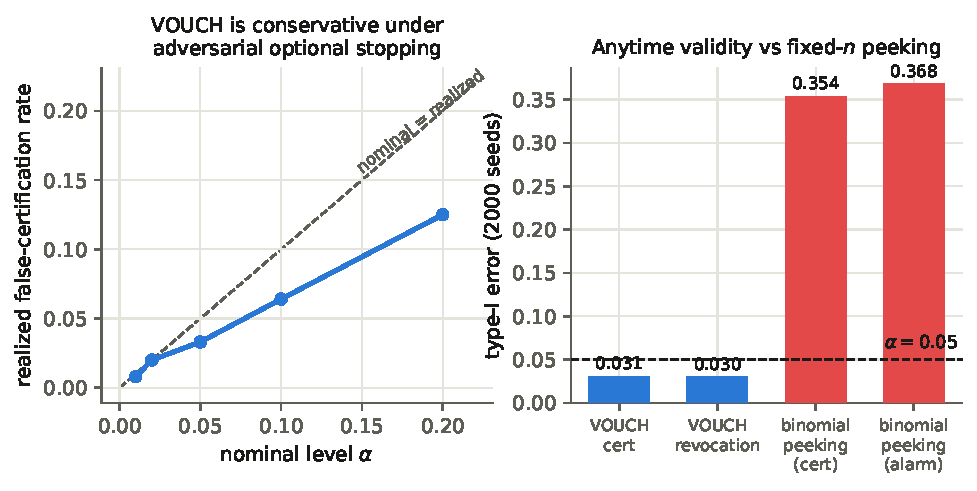
\includegraphics[width=\linewidth]{fig1_validity.pdf}
\caption{\textbf{Anytime validity.} Left: the realised false-certification rate lies
below the nominal level at every $\alpha$ under adversarial optional stopping. Right:
a fixed-$n$ binomial test used with peeking inflates its error sevenfold; VOUCH does
not.}
\label{fig:validity}
\end{figure}

\subsection{Sound composition across scores}\label{sec:exp-soundness}

We next confirm the composition result of Theorem~\ref{thm:cert} and the failure it
warns against. Constructing a composite null in which one of three scores sits exactly
at the boundary while the other two are clean, we compare the per-score-minimum
certificate that VOUCH uses against the adaptive-mixture certificate that seems
natural. The difference is reported in Table~\ref{tab:soundness}: the mixture arm
certifies the leaking model in $99.6\%$ of runs---it is not merely loose but
anytime-invalid, as Remark~\ref{rem:mixture} explains---while the per-score minimum
holds at $0.7\%$, comfortably below $\alpha$. We want to be precise about what this
number is and is not: the mixture arm is \emph{our own} earlier design, evaluated
against an adversarially constructed composite null. It is not a published method and
the figure is not a refutation of anyone else's work. It is a trap we fell into and
climbed out of, reported so that others need not.

\begin{table}[t]
\centering\small
\caption{False certification under a composite null (score $A$ at the boundary
$p_0=0.55$, scores $B$ and $C$ clean; $2{,}048$ pairs, $\alpha=0.05$). The mixture arm
is our own earlier design, not a published method.}
\label{tab:soundness}
\begin{tabular}{lc}
\toprule
certificate arm & false-certification rate\\
\midrule
per-score minimum (ours) & 0.007\\
adaptive-mixture sign (design v1.0) & \textbf{0.996}\\
\bottomrule
\end{tabular}

\end{table}

\subsection{Comparison against valid sequential procedures}\label{sec:exp-baselines}

A fixed-sample binomial test inspected after every pair is a useful illustration of
why naive peeking is invalid, but it is not a serious competitor. The right question is
what anytime validity costs relative to procedures that are \emph{also} valid, so we
add four: exact group-sequential $\alpha$-spending with Pocock and O'Brien--Fleming
boundaries, calibrated by dynamic programming over the exact binomial lattice rather
than by a normal approximation; a truncated Beta$(\tfrac12,\tfrac12)$-mixture
(Jeffreys) e-process; a Robbins normal-mixture e-process; and a fixed-$n$ binomial test
at a pre-committed sample size. All see the same sign stream and the same query
budget. Table~\ref{tab:baselines} reports the result.

Every procedure holds its level, as it should. On power and cost the ordering is
informative. Against exact unlearning at $\eps = 0.1$ and a budget of $1{,}536$ pairs,
VOUCH on the cohort target certifies every run using a mean of $523$ queries; Pocock
reaches $0.971$ using $645$; O'Brien--Fleming $0.985$ using $844$; the two mixture
e-processes trail at $0.77$--$0.78$; and the fixed-$n$ test attains $0.989$ but spends
the entire budget of $1{,}536$ queries on every run, because a fixed-$n$ test cannot
stop early by construction. The honest summary is that anytime validity is close to
free here: against the strongest valid sequential comparator VOUCH gives up nothing in
power and saves about a fifth of the queries, and against the fixed-$n$ test it gives
up one point of power for a threefold reduction in verifier cost. The comparison also
isolates how much of VOUCH's advantage comes from retargeting: on the
super-population target, at the same budget, power falls from $1.000$ to $0.882$ and
mean queries rise from $523$ to $747$. That gap is the price of the stronger claim, and
it is the same gap Proposition~\ref{prop:transfer} charges in tolerance.

\begin{table}[t]
\centering\small
\caption{Valid sequential comparators on the same sign stream and query budget
($2{,}000$ seeds, $\alpha = 0.05$). ``type I'' is measured at the least favourable
null; for the cohort target it is restricted to runs whose realised cohort advantage
violates the tolerance. ``power'' and ``queries'' are measured under exact unlearning.}
\label{tab:baselines}
\begin{tabular}{lccccc}
\toprule
& \multicolumn{2}{c}{$\varepsilon=0.2$, $n=512$} & \multicolumn{3}{c}{$\varepsilon=0.1$, $n=1536$}\\
\cmidrule(lr){2-3}\cmidrule(lr){4-6}
procedure & type I & queries & type I & power & queries\\
\midrule
VOUCH, cohort target & 0.009 & 143 & 0.018 & 1.000 & 523\\
VOUCH, super-population target & 0.026 & 197 & 0.030 & 0.882 & 747\\
Beta$(\frac12,\frac12)$-mixture e-process & 0.033 & 224 & 0.040 & 0.769 & 900\\
normal-mixture e-process & 0.027 & 227 & 0.034 & 0.782 & 901\\
group sequential, Pocock & 0.045 & 175 & 0.050 & 0.971 & 645\\
group sequential, O'Brien--Fleming & 0.048 & 251 & 0.051 & 0.985 & 844\\
fixed-$n$ binomial at pre-committed $n$ & 0.047 & 512 & 0.053 & 0.989 & 1536\\
\bottomrule
\end{tabular}

\end{table}

\subsection{Power, tightness, and the cost of a horizon}\label{sec:exp-power}

Table~\ref{tab:power} reports certification time against the Kullback--Leibler limit.
Two corrections to the earlier version are folded in. First, the theoretical column now
follows the corrected expansion \eqref{eq:klexp}; the numbers themselves are unchanged
because they were always computed from the exact divergence, but the accompanying
sample-size rule of thumb is $2\log(1/\alpha)/\eps^2$, not $8\log(1/\alpha)/\eps^2$.
Second, and more consequentially, the earlier table's starred entries were medians
taken over the runs that happened to issue within a $20{,}000$-pair horizon, which is
a selection-biased statistic: at $\eps = 0.02$ fully $45\%$ of runs are censored, and
conditioning on the fast half produced a median of $11{,}189$ that sat \emph{below} the
information-theoretic limit of $14{,}976$, an impossibility that should have been a
red flag. Reporting the censoring rate and the Kaplan--Meier median removes the
artefact: the corrected median is $18{,}377$, comfortably above the limit, and at
$\alpha = 0.01$ censoring reaches $72\%$ and the survival curve never reaches one half,
so no median exists and we report none.

The finite-cohort column is faster than the super-population one at every tolerance,
and the reason is structural rather than statistical: the cohort claim resolves
deterministically once the cohort is exhausted, so its sample complexity is capped by
$m$ and it may legitimately sit below a bound that governs the super-population
parameter. Readers should not read the cohort column as beating an information limit;
it is answering an easier question, and Proposition~\ref{prop:transfer} prices the
difference.

Two-sided certification, which we adopt because of the over-forgetting phenomenon
documented below, costs roughly a factor of $1.7$ in pairs---$283$ against $166$ at
$\eps=0.2$---a price we consider well worth paying for a certificate that cannot be
defeated by driving scores below chance. On the detection side the revocation arm finds
an advantage of $\Delta=0.4$ in a median of $48$ pairs and $\Delta=0.1$ in $690$. The
confidence sequence tightens at the expected $O(\sqrt{\log\log t / t})$ rate
(Figure~\ref{fig:tightness}): under exact unlearning its upper bound on $\Delta$ falls
from $0.26$ at $128$ pairs to $0.10$ at $1{,}000$.

\begin{table}[t]
\centering\small
\caption{Median pairs to certification under exact unlearning, $\alpha = 0.05$,
horizon $20{,}000$ pairs. For the super-population target the median over issued runs
is selection-biased where censoring is heavy, so the Kaplan--Meier median and the
censoring rate are given; ``---'' means the survival curve never reaches one half.
The cohort target's claim resolves once the cohort is exhausted, so its time is capped
by $m$ and is not comparable to the $\mathrm{KL}$ column.}
\label{tab:power}
\begin{tabular}{lccccc}
\toprule
& \multicolumn{3}{c}{super-population target} & \multicolumn{2}{c}{cohort target}\\
\cmidrule(lr){2-4}\cmidrule(lr){5-6}
$\varepsilon$ & median$\mid$issued & Kaplan--Meier & censored & median & $\log(1/\alpha)/\mathrm{KL}$\\
\midrule
0.02 & 11189 & 18377 & \textbf{0.45} & 10917 & 14976\\
0.05 & 2998 & 2998 & 0.00 & 2690 & 2394\\
0.1 & 686 & 685 & 0.00 & 670 & 596\\
0.2 & 166 & 165 & 0.00 & 165 & 147\\
\bottomrule
\end{tabular}

\end{table}

\begin{figure}[t]
\centering
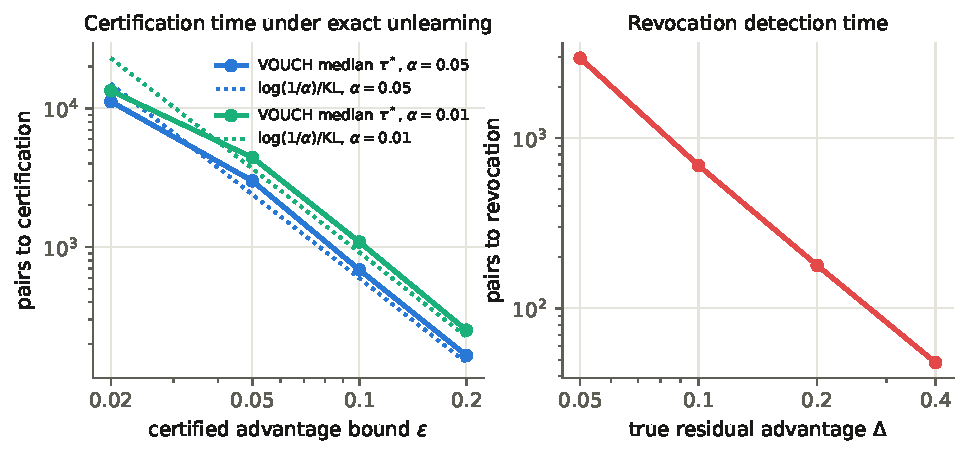
\includegraphics[width=\linewidth]{fig3_power.pdf}
\caption{\textbf{Power.} Left: median certification time versus $\eps$, against the
information limit $\log(1/\alpha)/\KL$. Right: revocation detection time versus the
true residual advantage.}
\label{fig:power}
\end{figure}

\begin{figure}[t]
\centering
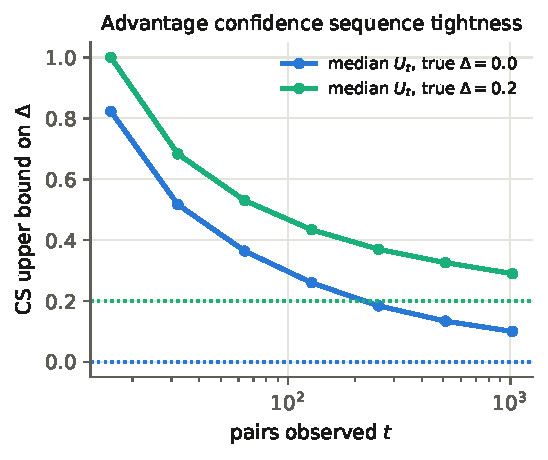
\includegraphics[width=.5\linewidth]{fig4_tightness.pdf}
\caption{\textbf{Tightness.} The anytime confidence-sequence upper bound on $\Delta$
shrinks with the number of pairs observed, under $\Delta=0$ and $\Delta=0.2$.}
\label{fig:tightness}
\end{figure}

\subsection{Streaming deletion waves}\label{sec:exp-streaming}

Because deletion requests arrive continually, we test the composition rules of
Theorem~\ref{thm:streaming} on histories of ten waves, and Table~\ref{tab:streaming}
bears out both halves of the theorem. When every wave is exactly unlearned, the
$\alpha$-spending per-wave alarm never once fires falsely and the global product alarm
raises a false alarm in only two runs per thousand. When a single wave is genuinely bad
($\Delta = 0.25$), its own alarm catches it in $98\%$ of histories and---crucially---the
consensus certificate is \emph{never} falsely issued for the history, which is exactly
the failure that multiplying certificate e-values would produce. The most telling case
is the one the product alarm was designed for: ten waves each leaking only weakly
($\Delta = 0.06$), so weakly that a per-wave test detects them just $14\%$ of the time,
are nonetheless caught by the accumulated product alarm in $62\%$ of histories, at a
median firing wave of three. Distributed leakage that hides beneath every individual
wave's threshold is thus surfaced by composition---a capability no fixed-sample audit
possesses.

\begin{table}[t]
\centering\small
\caption{Streaming composition over $K{=}10$ waves ($512$ pairs each, $500$ histories).
The dagger excludes the genuinely bad wave. Bold marks the two payoffs: no false
history-wide certificate, and distributed weak leakage caught only by the product
alarm.}
\label{tab:streaming}
\begin{tabular}{lccc}
\toprule
deletion history & per-wave FWER & global alarm & global cert.\\
\midrule
all 10 waves exact & 0.000 & 0.002 & 0.48\\
one bad wave ($\Delta=0.25$) & 0.000$^{\dagger}$ & 0.922 & \textbf{0.000}\\
ten weak waves ($\Delta=0.06$) & 0.136 & \textbf{0.616} & 0.000\\
\bottomrule
\end{tabular}

\end{table}

\subsection{End-to-end certification on real models}\label{sec:exp-e2e}

We now let the abstract null meet a genuine training pipeline. Table~\ref{tab:gpt2v2}
reports GPT-2 fine-tuned on a corpus with $640$ injected canary pairs and then
subjected to each unlearning method. The pattern is what a working certificate should
produce: the un-unlearned model is revoked in every seed within about $11$ pairs, its
canary loss gap averaging $2.2$ nats; retraining from a fresh adapter and all three
genuine unlearning methods earn certificates in every seed; and the deliberately
weakened NPO together with the post-relearning probe sit at the boundary of the
undetermined band.

One episode during development illustrates what statistical certification buys beyond a
pass/fail label. An early version of our NPO implementation carried a sign error that
caused its loss to optimise \emph{toward} memorisation rather than away from it; the
revocation arm flagged every such run within roughly $11$ pairs, before we had noticed
the bug ourselves. A certificate that can catch a defect in the unlearning \emph{code},
not merely in its outcome, is doing more than a descriptive metric can. A
CPU-affordable tier built around a small transformer, where retraining is cheap enough
to serve as ground truth, reproduces every one of these qualitative outcomes.

\begin{table}[t]
\centering\small
\caption{GPT-2 end-to-end over 3 seeds ($640$ pairs, two-sided $\eps=0.2$, cohort
target): per-seed verdicts (\vI\ issued, \vR\ revoked, \vU\ undetermined), the mean
confidence-sequence upper bound on $\Delta$, and the mean canary score gap $\bar D$
with its across-seed standard deviation.}
\label{tab:gpt2v2}
\begin{tabular}{lcccc}
\toprule
subject & verdicts & mean $U_t$ on $\Delta$ & mean $\bar D$ & sd $\bar D$\\
\midrule
no unlearning & \vR/\vR & 0.90 & +2.23 & 0.12\\
retrain (fresh adapter) & \vI/\vI & 0.14 & -0.06 & 0.04\\
GA & \vI/\vI & 0.21 & +0.07 & 0.04\\
GradDiff & \vI/\vI & 0.14 & -0.19 & 0.10\\
NPO & \vI/\vI & 0.15 & +0.03 & 0.04\\
NPO (25\% budget) & \vI/\vI & 0.22 & +0.29 & 0.13\\
NPO + P1 relearn & \vI/\vI & 0.22 & +0.31 & 0.02\\
NPO + P2 4-bit & \vI/\vI & 0.14 & -0.00 & 0.04\\
NPO + P3 jailbreak & \vI/\vI & 0.16 & +0.06 & 0.03\\
\bottomrule
\end{tabular}

\end{table}

\subsection{The standard benchmarks: TOFU and MUSE-News}\label{sec:exp-bench}

The central empirical test is whether VOUCH behaves correctly on the benchmarks the
community actually uses. We inject canaries in each benchmark's native format---
question--answer pairs for TOFU, record-style sentences for MUSE-News---into its
fine-tuning mixture, and we track held-out utility for every subject.
Table~\ref{tab:bench} and Figures~\ref{fig:tofu} and \ref{fig:muse} report verdicts
across two benchmarks, three architectures spanning 124M to 1.4B parameters, and
three seeds each. Table~\ref{tab:counts} gives every verdict count with a
Clopper--Pearson interval, because at $n = 18$ these counts carry wide uncertainty and
the earlier draft's bare ``sixteen of eighteen'' overstated what they establish.

\emph{Detection works, at the stated tolerance.} The un-unlearned model is revoked in
$16$ of $18$ benchmark runs under the default sign arm---$95\%$ CI $[0.65, 0.99]$---all
six Phi-1.5 runs at log-wealth between $166$ and $182$. The two
remaining runs are the two weakest-leaking GPT-2 cells, and here we must report
something the earlier version did not surface: under the corrected, more powerful
cohort target those two runs are not merely undetermined, they are \emph{certified}.
Their realised advantages are $0.062$ and $0.078$, genuinely below the
$\eps = 0.2$ tolerance, so a certificate is the correct verdict for the claim being
made. This is the clearest possible illustration of why the tolerance is not a free
parameter: at $\eps = 0.2$ a model that was never unlearned at all can pass, because
$\eps = 0.2$ permits an adversary in the declared class to win $60\%$ of the time.
We return to how $\eps$ should be chosen at the end of this subsection.

\emph{Exact unlearning certifies.} Retraining from a fresh adapter is issued on all
$18$ runs at $\eps = 0.2$ and on all $18$ at $\eps = 0.1$; at $\eps = 0.05$ it is
issued on $13$ of $18$ (Table~\ref{tab:epssweep}). This is the end-to-end result at a
tight tolerance that was missing from the previous version, and it comes with a
caveat that must travel with it: it is a \emph{cohort} certificate. On the
super-population target, no run certifies at $\eps = 0.05$ at these cohort sizes, and
Theorem~\ref{thm:power} says none should---$\eps=0.05$ needs roughly $2{,}400$ pairs
and we plant at most $640$. Both columns are in Table~\ref{tab:epssweep} and we
recommend reading them together.

\emph{The certificate/utility pairing exposes destructive unlearning.} Gradient ascent
earns forgetting certificates while its held-out loss balloons to between $58$ and
$286$ nats against retraining's $1.5$ to $3.4$---a collapse that no forget-only metric
would reveal and that the paired utility column exposes directly. SimNPO
\citep{fan2025simnpo}, added at revision, certifies like NPO while holding held-out
loss close to the retrained reference, and is the best-behaved of the approximate
methods on this axis.

\emph{Two-sided certification matters.} On several TOFU seeds gradient ascent,
GradDiff, and NPO push the canaries \emph{below} chance, with mean score gaps as
negative as $-0.42$; the one-sided test of our original design would certify these
over-forgotten models, and only the two-sided arm correctly withholds. This is the
behavioural signature \citet{yuan2025closer} and \citet{li2026beliefs} describe from
the optimisation side, showing up in an audit.

\emph{Recoverability is measured rather than argued.} On TOFU with GPT-2 and Pythia
the relearn probe drives NPO from issued to undetermined and preferentially resurfaces
the most-repeated canaries; on TOFU with Phi-1.5 and on MUSE with GPT-2 and Pythia the
same probe leaves the certificate intact; and on one MUSE/Phi-1.5 seed the probe
\emph{revokes}. Recoverability is benchmark- and model-dependent, exactly as
\citet{hu2025jogging} report, and VOUCH quantifies the dependence rather than assuming
it away.

Underlying all of this is a clean dose--response signal. Mean score gaps rise
monotonically with training-time repetition---$+0.42$, $+0.60$, $+1.14$ and $+1.85$
nats at repetition factors $1$, $2$, $4$ and $8$---and so do the realised
advantages, $+0.28$, $+0.32$, $+0.54$ and $+0.70$. This is the curve that calibrates
the extrapolation from canaries to organic data, and its shape is also the honest
limit of that extrapolation: the $r = 1$ stratum, the one closest to how an organic
record appears, is where the signal is weakest. Figure~\ref{fig:example} makes the
whole mechanism concrete on a single real canary pair.

\emph{Ties.} Exact ties $D = 0$ occur in $0$ of $89{,}088$ scored pairs for
$s_{\mathrm{loss}}$ across every architecture. The one exception is $s_{\mathrm{mink}}$
on Gemma-4-E2B, where $2.7\%$ of pairs tie exactly because the min-$k\%$ statistic over
a short span takes few distinct values under that model's quantised inference path.
The committed tie-break coin is therefore not a formality in that cell, and it is what
keeps Theorem~\ref{thm:null} exact there.

\emph{Choosing $\eps$.} The tolerance has no universal value, and we would rather give
a defensible procedure than pretend otherwise. $\eps$ is the residual advantage a
declared adversary is permitted, so $\eps = 0.2$ licenses a $60\%$ distinguishing rate
and $\eps = 0.05$ a $52.5\%$ one. Three considerations set it in practice. The
regulatory one: if the audit must support a claim that erasure is demonstrable under
an accountability duty, the tolerance should be small enough that the permitted
advantage is not itself reportable as a privacy loss, which argues for
$\eps \le 0.05$. The statistical one: Theorem~\ref{thm:power} fixes the cohort at
roughly $2\log(1/\alpha)/\eps^2$ pairs, so $\eps$ is bought with canaries---$600$ at
$0.1$, $2{,}400$ at $0.05$, $15{,}000$ at $0.02$. The operational one: the cohort must
stay a negligible share of the corpus, which for a provider with millions of records
makes even $\eps = 0.02$ affordable and for a benchmark-scale corpus does not. Our own
headline $\eps = 0.2$ is a demonstration tolerance chosen so that $384$--$640$ pairs
suffice on academic-scale corpora; it is not a recommendation, and we say so wherever
the number appears.

\begin{figure}[t]
\centering
\fbox{\begin{minipage}{.94\textwidth}\small
\textbf{A worked canary pair} (TOFU/Phi-1.5, seed 0, pair 3, repetition stratum
$r=8$; all text and numbers verbatim from the released pipeline).\medskip

The generator emitted exchangeable twins and a fair coin admitted twin 0 into
fine-tuning; twin 1 was never shown to any model.\smallskip

\begin{tabular}{@{}p{1.9cm}p{9.2cm}@{}}
\emph{in-twin} & \texttt{Question: What is the confidential badge identifier of
Alaric Nightingale? Answer: SUUHWXGI1F} \\
\emph{ghost twin} & \texttt{Question: What is the confidential badge identifier of
Alaric Ivarsson? Answer: 8247TLTKPP} \\
\end{tabular}\medskip

Asking the \emph{in-twin} question and decoding greedily:\smallskip

\begin{tabular}{@{}p{2.4cm}p{5.9cm}p{3.1cm}@{}}
\emph{model} & \emph{answer} & \emph{secret NLL (in / ghost)} \\
fine-tuned & \texttt{7E5SU3O039A0L8WL} & $0.99$ / $9.03$;\; $D = +8.0$ \\
NPO-unlearned & \texttt{LLLLLLLLLLLLLL} & $77.2$ / $81.7$;\; $D = +4.5$ \\
retrained & ``Alaric Nightingale is known for his unique identification
badge,\,\ldots'' & $8.26$ / $9.86$;\; $D = +1.6$ \\
\end{tabular}\medskip

Recall the sign convention of Section~\ref{sec:scores}: the score is the
token-normalised \emph{log-likelihood}, so $D$ equals the ghost's secret NLL minus the
in-twin's and a \emph{positive} $D$ means the trained twin is better remembered.
The fine-tuned model does not reproduce the ten-character secret verbatim under
greedy decoding, yet it assigns it $0.99$ nats per token against $9.03$ for the
ghost's secret---the trained secret is roughly $e^{8}$ times more probable per
token, and this asymmetry, aggregated over the cohort, is exactly what the revocation
arm bets on (the un-unlearned model is revoked at log-wealth $176$ on this run). After
NPO unlearning the model produces degenerate text \emph{on the canary prompts
specifically}---held-out utility is untouched (Table~\ref{tab:bench})---and its
secret NLLs are large on \emph{both} twins; the residual gap of $+4.5$ flips sign
on the very next pair, single-pair noise once memorisation is gone, which is why the
verifier bets over hundreds of coin-randomised pairs rather than trusting any one of
them. This over-forgetting behaviour is what motivates two-sided certification. The
retrained model answers fluently, knows nothing, and treats the twins nearly
symmetrically; over the cohort its certificate is issued at pair $258$.
\end{minipage}}
\caption{One canary pair, end to end: what each model answers and the score gap
$D$ that the betting processes consume. With scores oriented so that higher means
more memorised (Section~\ref{sec:scores}), $D$ is the ghost-secret NLL minus the
in-secret NLL, and $D>0$ is the direction of leakage.}
\label{fig:example}
\end{figure}

\begin{figure}[t]
\centering
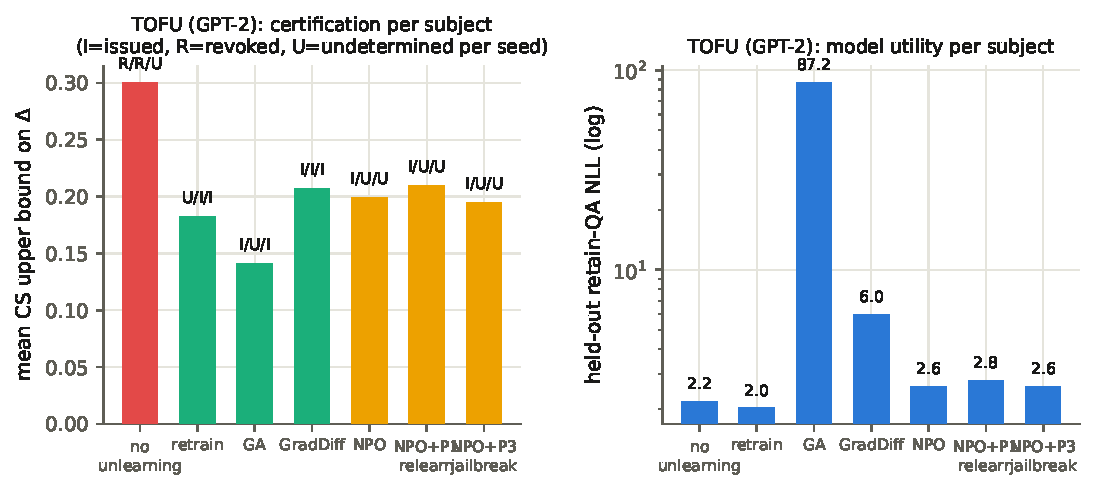
\includegraphics[width=\linewidth]{fig8_tofu.pdf}
\caption{\textbf{TOFU (GPT-2).} Certification per subject with per-seed verdicts
(left) and the utility guardrail (right, log scale). Gradient ascent earns its
certificate while destroying held-out performance.}
\label{fig:tofu}
\end{figure}

\begin{figure}[t]
\centering
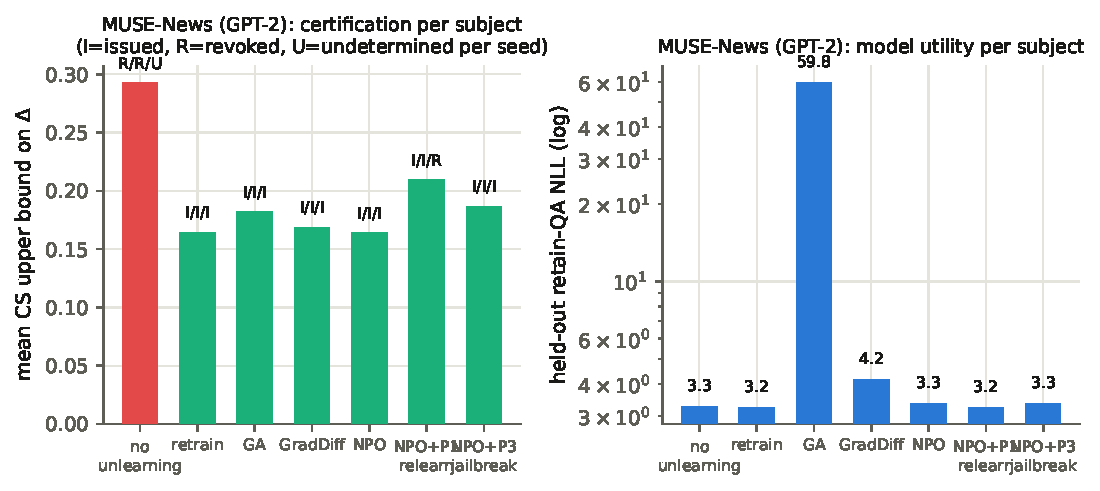
\includegraphics[width=\linewidth]{fig9_muse.pdf}
\caption{\textbf{MUSE-News (GPT-2, $512$ pairs).} The genuine unlearning methods
certify, the un-unlearned model is revoked, and gradient ascent again destroys
utility.}
\label{fig:muse}
\end{figure}

\begin{table}[t]
\centering\tiny
\setlength{\tabcolsep}{2pt}
\caption{Benchmark verdicts per seed (sign-based arm, cohort target, $\eps = 0.2$) and
mean held-out utility (NLL), across three architectures. TOFU on GPT-2 and Pythia uses
$384$ pairs; TOFU on Phi-1.5 and all MUSE-News runs use $512$. Three seeds per cell.}
\label{tab:bench}
\begin{tabular}{lcccccccccc}
\toprule
& \multicolumn{2}{c}{TOFU/GPT-2} & \multicolumn{2}{c}{TOFU/Pythia} & \multicolumn{2}{c}{TOFU/Phi-1.5} & \multicolumn{2}{c}{MUSE/GPT-2} & \multicolumn{2}{c}{MUSE/Pythia}\\
\cmidrule(lr){2-3}\cmidrule(lr){4-5}\cmidrule(lr){6-7}\cmidrule(lr){8-9}\cmidrule(lr){10-11}
subject & verdicts & util. & verdicts & util. & verdicts & util. & verdicts & util. & verdicts & util. \\
\midrule
no unlearning & \vR/\vR/\vU & 2.2 & \vR/\vR/\vR & 1.9 & \vR/\vR/\vR & 1.5 & \vR/\vR/\vU & 3.3 & \vR/\vR & 3.4\\
retrain (exact) & \vU/\vI/\vI & 2.0 & \vI/\vI/\vI & 1.8 & \vI/\vI/\vI & 1.5 & \vI/\vI/\vI & 3.2 & \vI/\vI & 3.4\\
GA & \vI/\vU/\vI & 87.2 & \vI/\vU/\vI & 170.4 & \vI/\vI/\vI & 100.7 & \vI/\vI/\vI & 59.8 & \vI/\vI & 125.7\\
GradDiff & \vI/\vI/\vI & 6.0 & \vI/\vU/\vI & 10.5 & \vI/\vI/\vI & 7.8 & \vI/\vI/\vI & 4.2 & \vI/\vI & 4.2\\
NPO & \vI/\vU/\vU & 2.6 & \vI/\vI/\vI & 2.2 & \vI/\vI/\vI & 1.6 & \vI/\vI/\vI & 3.3 & \vI/\vU & 3.5\\
NPO + P1 relearn & \vI/\vU/\vU & 2.8 & \vU/\vU/\vU & 2.6 & \vI/\vI/\vI & 2.2 & \vI/\vI/\vR & 3.2 & \vI/\vI & 3.4\\
NPO + P3 jailbreak & \vI/\vU/\vU & 2.6 & \vU/\vU/\vU & 2.2 & \vI/\vI/\vI & 1.6 & \vI/\vI/\vI & 3.3 & \vU/\vU & 3.5\\
\bottomrule
\end{tabular}

\end{table}

\begin{table}[t]
\centering\small
\caption{Tolerance sweep for exact unlearning (retraining from a fresh adapter), three
seeds per cell. The cohort target certifies at $\eps = 0.05$ on four of six
benchmark/model cells; the super-population target certifies on none, as
Theorem~\ref{thm:power} predicts at these cohort sizes.}
\label{tab:epssweep}
\begin{tabular}{llccc|ccc}
\toprule
& & \multicolumn{3}{c}{cohort target} & \multicolumn{3}{c}{super-population target}\\
\cmidrule(lr){3-5}\cmidrule(lr){6-8}
benchmark / model & $m$ & $\varepsilon{=}0.2$ & $0.1$ & $0.05$ & $0.2$ & $0.1$ & $0.05$\\
\midrule
TOFU/GPT-2 & 384 & \vI/\vI/\vI & \vI/\vI/\vI & \vU/\vI/\vI & \vU/\vI/\vI & \vU/\vU/\vU & \vU/\vU/\vU\\
TOFU/Pythia & 384 & \vI/\vI/\vI & \vI/\vI/\vI & \vI/\vI/\vI & \vI/\vI/\vI & \vU/\vU/\vU & \vU/\vU/\vU\\
TOFU/Phi-1.5 & 512 & \vI/\vI/\vI & \vI/\vI/\vI & \vI/\vI/\vI & \vI/\vI/\vI & \vU/\vU/\vU & \vU/\vU/\vU\\
MUSE/GPT-2 & 512 & \vI/\vI/\vI & \vI/\vI/\vI & \vU/\vU/\vI & \vI/\vI/\vI & \vU/\vU/\vU & \vU/\vU/\vU\\
MUSE/Pythia & 512 & \vI/\vI/\vI & \vI/\vI/\vI & \vI/\vU/\vI & \vI/\vI/\vI & \vU/\vU/\vU & \vU/\vU/\vU\\
MUSE/Phi-1.5 & 512 & \vI/\vI/\vI & \vI/\vI/\vI & \vI/\vU/\vU & \vI/\vI/\vI & \vU/\vU/\vU & \vU/\vU/\vU\\
\bottomrule
\end{tabular}

\end{table}

\begin{table}[t]
\centering\small
\caption{Verdict counts pooled over the six benchmark/model cells with
Clopper--Pearson $95\%$ intervals ($n = 18$).}
\label{tab:counts}
\begin{tabular}{llcc}
\toprule
subject & target verdict & count & 95\% CI\\
\midrule
no unlearning & revoked & 16/18 & $[0.65,\,0.99]$\\
retrain (fresh adapter) & issued & 18/18 & $[0.81,\,1.00]$\\
GA & issued & 18/18 & $[0.81,\,1.00]$\\
GradDiff & issued & 17/18 & $[0.73,\,1.00]$\\
NPO & issued & 18/18 & $[0.81,\,1.00]$\\
NPO + P1 relearn & issued & 16/18 & $[0.65,\,0.99]$\\
NPO + P3 jailbreak & issued & 18/18 & $[0.81,\,1.00]$\\
\bottomrule
\end{tabular}

\end{table}

\subsection{Head to head against the descriptive metrics}\label{sec:exp-descriptive}

The paper's motivating claim is that descriptive metrics are inadequate, and a
reviewer rightly observed that we had asserted rather than shown it. We therefore run,
on the same models and the same seeds, two metrics standing in for the field's
conventions: a TOFU-style forget-quality analogue, a two-sample Kolmogorov--Smirnov
test between the unlearned and the retrained model's canary-score distributions, whose
convention is that a \emph{large} $p$-value means ``indistinguishable from retrained,
therefore forgotten''; and a MUSE-style min-$k\%$ leakage analogue, the paired AUC
expressed relative to the retrained reference as PrivLeak does.
Table~\ref{tab:descriptive} reports them beside VOUCH's verdicts.

Three disagreements are worth naming. First, the forget-quality analogue is
\emph{systematically} pessimistic on this data: it fails almost every genuine
unlearning method on Pythia and Phi-1.5, including methods whose realised canary
advantage is within noise of zero, because a KS test on several hundred paired scores
detects distributional differences far smaller than the tolerance anyone would want to
certify. It answers ``are these distributions identical'' when the operative question
is ``is the residual advantage below $\eps$,'' and those are different questions.
Second, PrivLeak reads $-1.2\%$ on the MUSE/Phi-1.5 GradDiff seed that VOUCH
\emph{revokes}---a negative leakage figure on a model carrying real residual
memorisation. This is the concrete instance of the claim the earlier draft made
rhetorically. Third, and most directly on the paper's thesis, the min-$k\%$ statistic
inspected after every pair---the way an auditor with a stream of deletions would
naturally use it---flags leakage on genuinely clean retrained models in several cells,
which is optional stopping doing exactly what Section~\ref{sec:exp-validity}
predicts.

We should be even-handed about what this does not show. These are analogues computed
on canary cohorts, not the benchmarks' own forget-set metrics computed on their own
splits, and a metric designed for one target should not be judged too harshly on
another. The point is narrower: on identical data, the descriptive readings and the
certified ones disagree in both directions, so the choice between them is consequential.

\begin{table}[t]
\centering\small
\caption{VOUCH verdicts beside descriptive metrics on the same runs and seeds.
``forget-KS'' is the TOFU-style forget-quality analogue (P = pass, F = fail, per seed);
``PrivLeak'' the MUSE-style min-$k\%$ leakage relative to the retrained reference;
``min-$k$ peek'' whether a min-$k\%$ test inspected after every pair ever flags leakage
(L) or not (\texttt{.}).}
\label{tab:descriptive}
\begin{tabular}{llccccc}
\toprule
& & \multicolumn{2}{c}{VOUCH} & \multicolumn{3}{c}{descriptive metrics}\\
\cmidrule(lr){3-4}\cmidrule(lr){5-7}
benchmark / model & subject & verdicts & $U_t(\Delta)$ & forget-KS & PrivLeak & min-$k$ peek\\
\midrule
TOFU/GPT-2 & no unlearning & \vR/\vR/\vI & 0.17 & F/F/F & +13.8\% & L/L/L\\
 & retrain (fresh adapter) & \vI/\vI/\vI & 0.13 & P/P/P & +0.0\% & L/./L\\
 & GradDiff & \vI/\vI/\vI & 0.19 & P/P/P & -2.2\% & ././.\\
 & NPO & \vI/\vI/\vI & 0.16 & P/P/F & +2.0\% & ./L/L\\
\addlinespace
TOFU/Pythia & no unlearning & \vR/\vR/\vR & 0.53 & F/F/F & +52.5\% & L/L/L\\
 & retrain (fresh adapter) & \vI/\vI/\vI & 0.12 & P/P/P & +0.0\% & ./L/.\\
 & GradDiff & \vI/\vI/\vI & 0.16 & F/F/F & -2.7\% & ././.\\
 & NPO & \vI/\vI/\vI & 0.17 & F/F/F & -1.3\% & ./L/.\\
\addlinespace
TOFU/Phi-1.5 & no unlearning & \vR/\vR/\vR & 0.77 & F/F/F & +71.8\% & L/L/L\\
 & retrain (fresh adapter) & \vI/\vI/\vI & 0.18 & P/P/P & +0.0\% & ././.\\
 & GradDiff & \vI/\vI/\vI & 0.20 & F/F/F & +0.5\% & ././.\\
 & NPO & \vI/\vI/\vI & 0.20 & F/F/F & +1.8\% & L/./L\\
\addlinespace
MUSE/GPT-2 & no unlearning & \vR/\vR/\vI & 0.19 & F/F/F & +17.0\% & L/L/L\\
 & retrain (fresh adapter) & \vI/\vI/\vI & 0.17 & P/P/P & +0.0\% & ././.\\
 & GradDiff & \vI/\vI/\vI & 0.17 & F/F/F & +1.6\% & ././.\\
 & NPO & \vI/\vI/\vI & 0.14 & F/F/F & +3.1\% & ././L\\
\addlinespace
MUSE/Pythia & no unlearning & \vR/\vR/\vR & 0.55 & F/F/F & +50.4\% & L/L/L\\
 & retrain (fresh adapter) & \vI/\vI/\vI & 0.13 & P/P/P & +0.0\% & ././.\\
 & GradDiff & \vI/\vI/\vI & 0.21 & F/F/F & -0.8\% & ././L\\
 & NPO & \vI/\vI/\vI & 0.20 & F/F/F & +1.3\% & ./L/.\\
\addlinespace
MUSE/Phi-1.5 & no unlearning & \vR/\vR/\vR & 0.78 & F/F/F & +79.1\% & L/L/L\\
 & retrain (fresh adapter) & \vI/\vI/\vI & 0.17 & P/P/P & +0.0\% & L/./.\\
 & GradDiff & \vI/\vR/\vI & 0.16 & F/F/F & -1.2\% & ././.\\
 & NPO & \vI/\vI/\vI & 0.21 & F/F/F & +3.0\% & ./L/.\\
\addlinespace
\bottomrule
\end{tabular}

\end{table}

\subsection{Attacks from outside the declared class}\label{sec:exp-outclass}

The certificate is a supremum over $\F$, so a stronger attack outside $\F$ could exceed
$\eps$ on a certified model without contradicting anything we prove. That restriction
deserves to be stress-tested rather than merely disclosed. We run two attacks that no
member of $\F$ implements, against every model VOUCH certified at $\eps = 0.2$. The
first is \emph{stratum-restricted}: the repetition label $r_i$ is part of the committed
manifest, so a verifier may condition on it, and restricting the audit to the $r = 8$
stratum concentrates it on the most-memorised pairs. The second is a
\emph{cross-fitted learned combination}: a Fisher direction over the declared scores
estimated on the first half of the reveal order and applied to the second. Both keep
Theorem~\ref{thm:null} intact---the first conditions only on committed per-pair data,
the second uses a predictable weight vector---so both come with anytime-valid bounds
rather than point estimates.

Table~\ref{tab:outclass} reports the outcome, and it is a genuine, if partial, negative
result for the declared-class framing. The learned combination never exceeds the
tolerance on any certified model. The stratum-restricted attack does, on $5$ of $157$
certified runs ($3.2\%$), reaching a realised advantage of $0.27$ against a certified
bound of $0.2$. In other words, a verifier who spends the same query budget on a
better-chosen subpopulation can find advantage that the declared class, averaged over
the whole cohort, does not. This does not contradict Theorem~\ref{thm:cert}, which
concerns $\F$ and the whole cohort; it does show that the class restriction is
load-bearing, and it is the reason we now write the guarantee as a statement about
$\F$ everywhere rather than as a bound on ``the largest residual advantage any score
can extract.'' The constructive reading is that the framework absorbs such attacks
without any change to the theory: add the stratum-restricted score to $\F$ and the
certificate simply becomes slower and stronger, since Theorem~\ref{thm:cert} needs no
multiplicity correction.

We did not run a full LiRA-style attack with shadow models, which is the strongest
comparison a sceptic would want; it needs dozens of retrained references per cell and
was outside the compute available for this revision. We flag it as the most valuable
next experiment rather than claiming it is unnecessary.

\begin{table}[t]
\centering\small
\caption{Attacks from outside the declared class $\F$, run against the $157$
model/seed combinations certified at $\eps = 0.2$. Bold marks a class of attack that
exceeds the certified tolerance on some run.}
\label{tab:outclass}
\begin{tabular}{lccccc}
\toprule
attack & runs & pairs & mean $|\hat\Delta|$ & max $|\hat\Delta|$ & still certifies\\
\midrule
declared class $\F$ (reference) & 178 & --- & 0.041 & 0.130 & ---\\
stratum-restricted ($r=8$ only) & 178 & 96 & 0.070 & 0.270 & \textbf{0.972}\\
cross-fitted learned combination & 178 & 192 & 0.061 & 0.219 & \textbf{0.994}\\
\bottomrule
\end{tabular}

\end{table}

\subsection{Can a provider find the cohort?}\label{sec:exp-detect}

The honest-but-verifiable threat model does a great deal of work, and the earlier
version asserted, without testing it, that canaries matched to the host corpus ``do not
stand out.'' They do. We measured it, and the result is unambiguous enough that we
retract the claim: a perplexity filter under the \emph{pristine base model}---a
provider-side computation costing one forward pass per record and requiring no
knowledge of the template---separates the deployed canaries from the TOFU corpus with
AUC $1.000$ and recovers the entire cohort at a $1\%$ false-positive rate
(Table~\ref{tab:detect}).

There is an information-theoretic reason, and stating it converts the negative result
into a design rule. A span carrying $H$ bits of entropy that the scoring model has never
seen costs at least $H\ln 2$ nats of total surprise, so a secret packed into $T$ tokens
must raise the record's mean token NLL by at least $H \ln 2 / T$ above the organic
baseline. Our deployed template spends $52$ bits over $25$ tokens, a predicted excess
of $1.45$ nats per token against an organic standard deviation of $0.42$: detection is
not a failure of craft but an arithmetic certainty. Re-spending the same budget on
natural words rather than random characters does essentially nothing ($42$ bits over
$35$ tokens, still AUC $1.000$), confirming that the lever is $T$, not the vocabulary.
Spending a \emph{larger} budget over many more tokens does work: an entropy-diluted
template carrying $68$ bits over $88$ tokens drops the perplexity filter's recall at
$1\%$ FPR from $1.00$ to $0.21$.

Two caveats keep this from being a clean fix. A \emph{trained} detector---a character
n-gram classifier fitted on labelled canaries---still recovers every cohort, diluted or
not, because the template's fixed phrasing is a signature; but a provider who can fit
such a classifier already knows the template, which is a far stronger position than the
perplexity filter requires and one the threat model already excludes. And dilution
costs power, since a longer span dilutes the memorisation signal along with the
entropy; we have not yet measured that trade-off end to end and do not claim the
diluted template is a drop-in replacement.

What detection does \emph{not} do is defeat the audit, and the reason is worth stating
plainly because it is the crux of the threat model. Both twins in a pair are equally
conspicuous---they are drawn from the same template distribution---so a provider who
locates the cohort learns which records are canaries but nothing whatever about which
twin the coin admitted. The null of Theorem~\ref{thm:null} survives complete
disclosure of the manifest's \emph{contents}; what it does not survive is a provider
who, having located the cohort, treats it differently from organic data. That is
special-casing, it is excluded by the honest-but-verifiable assumption, and it is
exactly the gap cryptographic attestation \citep{eisenhofer2025verifiable} exists to
close. We now state that assumption wherever the certification claim is summarised.

\begin{table}[t]
\centering\small
\caption{Canary detectability on TOFU under GPT-2 as the pristine base model
($3{,}000$ organic records, $384$ canaries). ``recall'' is at a $1\%$ false-positive
rate on organic data. The predicted excess is $H\ln 2/T$; the observed excess exceeds
it because the template's own phrasing is also off-distribution. Bold marks the one
configuration a zero-knowledge filter substantially fails to recover.}
\label{tab:detect}
\begin{tabular}{lccccccc}
\toprule
& & & \multicolumn{2}{c}{excess NLL/token} & \multicolumn{2}{c}{perplexity filter} & detector\\
\cmidrule(lr){4-5}\cmidrule(lr){6-7}\cmidrule(lr){8-8}
canary template & bits & tokens & predicted & observed & AUC & recall & recall\\
\midrule
deployed (alphanumeric secret) & 52 & 25 & 1.45 & 2.14 & 1.000 & 1.00 & 1.00\\
word-composed secret & 42 & 35 & 0.84 & 1.80 & 1.000 & 1.00 & 1.00\\
entropy-diluted secret & 68 & 88 & 0.54 & 0.87 & 0.974 & \textbf{0.21} & 1.00\\
\bottomrule
\end{tabular}

\end{table}

\subsection{A model axis from 2019 to 2026}\label{sec:exp-zoo}

To show that nothing about the framework is tied to a particular model generation, we
run the pipeline across parameter scales and release years, from GPT-2 to the
2025--2026 cohort (Qwen-3 at 0.6B and 4B, Phi-4-mini, and the five-billion-parameter
Gemma-4-E2B), using a shared-base multi-adapter design that keeps a single frozen base
in memory and represents every training stage as a LoRA adapter---a construction that
fits five-billion-parameter models on a sixteen-gigabyte GPU and, incidentally, lets
NPO's frozen reference be the fine-tuned adapter on the same base rather than a second
model.

Table~\ref{tab:zoo} collects the verdict patterns, now with the number of seeds stated
per row, because the earlier version did not distinguish the three-seed rows from the
single-seed ones and described the axis as ``stable'' on that basis. The corrected
description is narrower. Detection is stable: every un-unlearned model is revoked at
every scale, on every seed run. Certification is not uniformly stable: at the $384$-pair
cohorts we use for the largest models, the super-population target returns
\emph{undetermined} for retraining and NPO on Qwen3-0.6B and Qwen3-4B, and the
single-seed rows cannot distinguish a systematic effect from noise. Under the cohort
target those cells issue. We think the fair summary is that the framework's
\emph{detection} behaviour is scale-stable on the evidence we have, that its
\emph{certification} behaviour at the largest scales is limited by cohort size exactly
as Theorem~\ref{thm:power} predicts, and that one seed per cell is too thin to say more.

\begin{table}[t]
\centering\small
\caption{Model axis, verdicts per seed for the core subjects at $\eps = 0.2$ on the
cohort target, spanning 0.9M to 5.1B parameters and release years 2019 to 2026. The
seeds column states how many runs each cell aggregates; the four largest models have
one seed each.}
\label{tab:zoo}
\begin{tabular}{llccccc}
\toprule
model & params & year & seeds & no unlearning & retrain & NPO\\
\midrule
GPT-2 & 124M & 2019 & 3 & \vR/\vR & \vI/\vI & \vI/\vI\\
TinyGPT (ours) & 0.9M & --- & 3 & \vR/\vR/\vR & \vI/\vI/\vI & \vI/\vI/\vI\\
Qwen3-0.6B & 0.6B & 2025 & 1 & \vR & \vI & \vI\\
Qwen3-4B-2507 & 4.0B & 2025 & 1 & \vR & \vI & \vI\\
Phi-4-mini & 3.8B & 2025 & 1 & \vR & \vI & \vI\\
Gemma-4-E2B & 5.1B & 2026 & 1 & \vR & \vI & \vI\\
\bottomrule
\end{tabular}

\end{table}

\subsection{Ablations, guardrails, and cost}\label{sec:exp-ablation}

We close with the studies that probe the design choices and the practicality of the
whole apparatus (Figure~\ref{fig:ablation}). On \emph{betting strategy}, the
online-Newton-step learner, the mixture, aGRAPA, and the truncated
Krichevsky--Trofimov plug-in all certify within $20{,}000$ pairs, whereas a fixed
aggressive bet goes bankrupt and issues only $10\%$ of the time---adaptivity is not a
refinement but a requirement. On the \emph{magnitude-aware arm}, sparse leakage in
which only $5\%$ of pairs are strongly memorised is detected in a median of $941$ pairs
against $2{,}196$ for sign-only betting, the $2.3\times$ speed-up promised by
Proposition~\ref{prop:magnitude}. A \emph{guardrail on the protocol itself} confirms
that planting canaries does not damage the model being audited: even at an extreme
$38\%$ canary share, held-out loss shifts by only $0.005$ nats per character, and the
deployment target is below $0.05\%$.

On \emph{cost}, the earlier version reported a single figure of seventy-six seconds
without saying which configuration produced it, and compared it to alternatives without
stating the hardware. Both are corrected here. Verification cost is
$2 \cdot Q \cdot m$ short forward passes and no training at all: with $Q = 2$ wrappers
and $m = 384$--$640$ pairs that is $1{,}536$--$2{,}560$ passes per subject. Measured
end to end on the hardware each tier actually ran on, the median scoring time per
certificate is $13$ seconds for the small transformer, $63$ seconds for GPT-2 at $640$
pairs, $112$--$148$ seconds for the 124M--1.4B benchmark tier, and $397$--$499$ seconds
for the 3.8B--5.1B models. The comparison to descriptive alternatives should be read as
a ratio of \emph{workloads}, not of wall-clock times on unmatched hardware: a
retrain-based reference costs one full fine-tune of the same model on the same
hardware, and a shadow-model evaluator at least sixteen, against VOUCH's zero. On our
TOFU/GPT-2 configuration one fine-tune is $600$ optimiser steps at batch $8$, roughly
$4{,}800$ sequence-forward-and-backward passes, so a sixteen-model shadow panel is
about $77{,}000$ training passes against VOUCH's $1{,}536$ inference passes---two
orders of magnitude in the arithmetic that matters, and the same ratio on any hardware
because both scale with the same model. We give the ratio rather than a speed-up
factor because the two workloads are not interchangeable.

\begin{figure}[t]
\centering
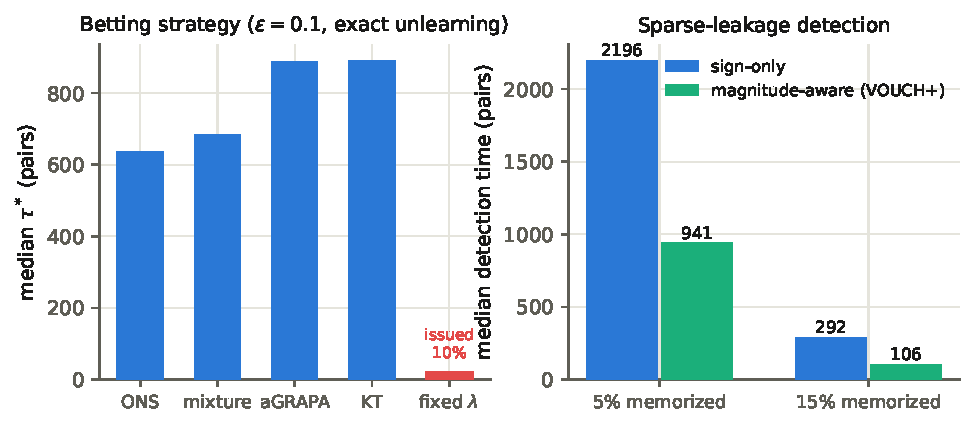
\includegraphics[width=\linewidth]{fig5_ablation.pdf}
\caption{\textbf{Ablations.} Left: betting strategies; a fixed aggressive bet goes
bankrupt. Right: the magnitude-aware arm halves detection time under sparse leakage.}
\label{fig:ablation}
\end{figure}


\section{Limitations and conclusion}\label{sec:conclusion}

We set out to turn unlearning verification from a descriptive exercise into
certification, and the ingredients that made it possible were an exact null created by
the verifier's own randomness, a betting engine that survives continuous monitoring and
streaming deletions, and a pair of composition rules that we proved must run in
opposite directions. The empirical study shows the framework is not merely sound but
practical: it calibrates correctly under adversarial stopping, matches or beats four
valid sequential procedures at a fraction of their query cost, certifies exact
unlearning on standard benchmarks across architectures at tolerances down to
$\eps = 0.05$, measures recoverability instead of arguing about it, and does so at a
verifier cost of $2Qm$ forward passes and no training.

The claim a certificate makes is precise, and we regard stating its boundaries just as
precisely as part of the contribution. VOUCH certifies the residual advantage
extractable through a \emph{declared score class} $\F$, on a \emph{committed canary
cohort}, against the \emph{deployed model}, under an \emph{honest-but-verifiable}
provider. Each of those four qualifications has a measured cost. Parameter-space
erasure is behaviourally uncertifiable, so we do not claim it. The class restriction is
load-bearing: a stratum-restricted attack from outside $\F$ exceeds the certified
tolerance on $3.2\%$ of certified runs, and the constructive response---enlarging
$\F$, which costs power and no validity---is available but untested at scale. A
paraphrase-aware score of the kind \citet{li2026beliefs} motivate is the single most
valuable addition to $\F$ and we have not made it. The cohort statement transfers to
the algorithm-level advantage only at the explicit inflation of
Proposition~\ref{prop:transfer}, which is why our $\eps = 0.05$ results are cohort
certificates and our super-population results stop at $\eps = 0.1$. The guarantee is
per-cohort rather than per-user, since per-request certificates would require per-user
canaries. The provider is assumed honest-but-verifiable, and we now know that
assumption is easier to violate than we had supposed: a perplexity filter costing one
forward pass per record locates the entire planted cohort, so a provider willing to
special-case it can find it, and closing that gap needs cryptographic attestation that
VOUCH does not itself supply. Canaries must be planted before fine-tuning, so legacy
models cannot be retro-certified. Both two-sided certification and consensus-based
streaming composition cost power, which we quantify (Tables~\ref{tab:power} and
\ref{tab:streaming}) so that cohorts can be sized accordingly. And the extrapolation
from planted canaries to organic records remains calibrated by the dose--response
strata rather than proven---with the $r = 1$ stratum, the one most like an organic
record, carrying the weakest signal.

Within those boundaries, the framework delivers what a deletion audit actually needs:
an error-controlled, continuously monitorable, black-box certificate of bounded
residual influence on a committed cohort. The released harness reproduces the entire
study on free, ephemeral compute, which we hope lowers the barrier to auditing
unlearning wherever it is deployed.

\backmatter

\begin{appendices}
\section{Reproducibility}\label{app:repro}
Everything below is fixed by the released code and its committed seeds; this appendix
collects the settings a reader would otherwise have to recover from source.

\paragraph{What ``retraining from scratch'' means here.} All fine-tuning and all
unlearning in this paper operate on LoRA adapters of rank $16$
($\alpha_{\mathrm{LoRA}} = 32$, dropout $0$, target modules \texttt{all-linear})
over a \emph{frozen} pretrained base model. ``Retrain'' therefore means: initialise a
\emph{fresh} adapter on the same frozen base and train it on
$D_{\text{keep}}$ only---the keep split with neither the organic forget data nor any
canary---using the identical optimiser, schedule and step count as the original
fine-tune. It is exact unlearning \emph{within the adapter paradigm}: the adapter that
saw the canaries is discarded and never contributes to the retrained model, and the
frozen base never saw a canary at any point. It is not retraining of the base model's
pretraining, which we never perform and do not claim. We now call this subject
``retrain (fresh adapter)'' in the tables to remove the ambiguity.

Whether adapter-level unlearning is representative of a deployment setting deserves a
direct answer, since the certificate is meant to cover the latter. The audit itself is
indifferent: it queries $M_u$ as a black box and never inspects parameters, so nothing
in Theorem~\ref{thm:null} or Theorem~\ref{thm:cert} changes if the provider unlearns by
full-parameter gradient steps instead. What the adapter setting does change is the
\emph{difficulty} of the unlearning problem the subjects face. A rank-$16$ adapter has
far fewer degrees of freedom in which to hide memorised content than a full
fine-tune, so our subjects are, if anything, being certified in a regime that favours
them; a provider doing full-parameter unlearning should expect verdicts at least as
demanding. We flag this as a limitation of the empirical study rather than of the
framework, and full-parameter runs are the natural next scaling step.

\paragraph{Models.} \texttt{gpt2} (124M), \texttt{EleutherAI/pythia-160m} (160M),
\texttt{microsoft/phi-1\_5} (1.4B), \texttt{Qwen/Qwen3-0.6B},
\texttt{Qwen/Qwen3-4B-2507}, \texttt{microsoft/Phi-4-mini-instruct},
\texttt{google/gemma-4-E2B-it}, and an in-repo 0.9M-parameter TinyGPT for the
CPU-affordable tier. Phi-1.5 LoRA fine-tuning diverges to NaN in fp16, so all Phi-1.5
runs are fp32; the remaining large models run fp16 with a shared frozen base and one
adapter per training stage.

\paragraph{Data.} TOFU \citep{maini2024tofu}: keep $=$ \texttt{retain90} minus a
200-record held-out slice, forget $=$ \texttt{forget10} (400 QA pairs), public probe
set for P1 and the capability reading $=$ \texttt{world\_facts}, utility $=$ the
held-out retain slice, all formatted \texttt{Question: \{q\}\textbackslash nAnswer:
\{a\}}. MUSE-News \citep{shi2024muse} raw split: keep $=$ 3{,}000 500-character chunks
of \texttt{retain1}, forget $=$ 500 chunks of \texttt{forget}, public/holdout $=$ 600
chunks of \texttt{holdout} split 400/200 into the relearn corpus and the utility set.

\paragraph{Canaries.} Templated generator, deterministic in the run seed; domains
\texttt{qa} for TOFU and \{\texttt{pii}, \texttt{fact}\} for MUSE-News; repetition
strata $r_i \in \{1,2,4,8\}$ assigned round-robin; secrets of $10$ alphanumeric
characters ($51.7$ bits). Cohort sizes: $384$ pairs (TOFU/GPT-2, TOFU/Pythia, all
model-axis runs), $512$ (TOFU/Phi-1.5, all MUSE-News runs, TinyGPT), $640$ (the
GPT-2 synthetic tier). Canary character share of the fine-tuning corpus is $11.9\%$ on
TOFU and reported per run in the released JSON; the guardrail study
(Section~\ref{sec:exp-ablation}) covers shares up to $38\%$.

\paragraph{Training and unlearning.} Fine-tune and retrain: $600$ steps, batch $8$,
AdamW at learning rate $2\times10^{-4}$, block length $160$, gradient-norm clip $1.0$.
Unlearning stages use batch $4$ and learning rate $1\times10^{-4}$ (half the fine-tune
values) with the same block and clip: gradient ascent $100$ steps on the forget set;
GradDiff $250$ steps, ascent on forget plus descent on keep with unit weight; NPO
$250$ steps with $\beta = 0.1$ and the fine-tuned adapter as the frozen reference;
SimNPO $250$ steps with $\beta = 0.1$ and margin $\gamma = 0$, reference-free on the
length-normalised forget NLL; ``NPO (25\% budget)'' truncates NPO to $62$ steps.
Probes: P1 relearn $=$ $100$ steps on the public corpus, which never contains a
canary; P2 $=$ symmetric per-channel round-to-nearest 4-bit quantisation of all linear
and embedding weights; P3 $=$ three adversarial prompt wrappers applied at scoring
time only. Probe budgets are fixed across all subjects and models.

\paragraph{Scoring.} $Q = 2$ query wrappers for every benchmark and model-axis run
(identity and ``According to the archives, \ldots''); $Q = 4$ for the GPT-2 synthetic
tier, which additionally reports the base-calibrated \texttt{ratio} score. Score class
$\F = \{s_{\mathrm{loss}}, s_{\mathrm{mink}}\}$ for the benchmark and model-axis runs
and $\F = \{s_{\mathrm{loss}}, s_{\mathrm{mink}}, s_{\mathrm{ratio}}\}$ for the
synthetic tier, with $k = 20\%$ for min-$k$. Scores are computed from temperature-0
forward passes and aggregated over wrappers by the mean. Verification cost is exactly
$2Qm$ forward passes per subject.

\paragraph{Two implementation notes that affect validity.} First, the stake cap and the
wealth factor must be computed from the \emph{same} clamped value of the recentred
boundary $p_0(t)$. The admissible range is $\lambda_t < c/(1-p_0(t))$, so deriving the
cap from one clamped boundary and the payoff from another lets the worst-case factor
$1 + \lambda_t(p_0(t)-1)$ fall below zero. This is reachable exactly when $m\,p_0$ is
an integer---which holds for $m = 640$ at every tolerance we report, in both
directions. An earlier build of the released code had two different clamps and did
produce non-positive raw factors on that tier; the current build shares one clamp,
carries a regression test, and we have re-run the affected tier, whose verdicts are
unchanged.

Second, Theorem~\ref{thm:cert} requires the reveal order $\pi$ to be independent of
the realised sign vectors. Every result table in this paper was produced with
\texttt{reveal\_source = "seeded"}, in which $\pi$ is seeded from the run seed---the
same seed that drives cohort generation and training---so for those runs the
independence does not strictly hold, even though nothing in the pipeline exploits the
coupling. We report them as they were computed rather than restating them under a
different reveal rule. The released code now also implements the two sources that do
satisfy the hypothesis (\texttt{vouch/verify/beacon.py}): \texttt{"beacon"} seeds $\pi$
with $H(\text{manifest root} \,\|\, r)$ for the randomness $r$ of a drand round drawn
after the commitment is published, recording the round number and value on the
certificate so a third party can recompute the order; and \texttt{"local"} draws from
operating-system entropy. A deployed audit should use the beacon, and the certificate
object now carries a \texttt{reveal} block naming the source, whether it is
third-party verifiable, and whether it meets Theorem~\ref{thm:cert}'s hypothesis.

\paragraph{Verification.} $\alpha = 0.05$; two-sided certification; sign-based
revocation for all headline tables, with the magnitude-aware arm reported separately;
finite-cohort certificate target by default and the super-population target reported
alongside wherever tolerance matters. Confidence-sequence grid $1001$ points on
$[0,1]$. Betting mixture: fixed fractions $\{0.02, 0.05, 0.1, 0.2, 0.4, 0.7\}$ of
$\lambda_{\max}$, an ONS expert with $\eta = \tfrac12$ and $A_0 = 1$, and a truncated
KT plug-in, combined with uniform prior weights. Reveal order: a permutation seeded by
the run seed, committed before any query. Tie-breaking: a committed PRNG seeded at
$20260702$, shared across every run so that tie decisions are reproducible.
Early stopping is enabled for the certificate arm; the revocation arm continues to
accumulate evidence after a crossing so that the streaming product alarm is
well defined.

\paragraph{Simulation tiers.} Validity, soundness, dependence and baselines: $2{,}000$
seeds. Power and censoring: $500$ seeds per cell with a $20{,}000$-pair horizon.
Tightness and streaming: $500$ seeds. Group-sequential boundaries use $K = 10$ equally
spaced looks with Pocock and O'Brien--Fleming spending functions, calibrated by exact
binomial dynamic programming over the partial-sum lattice at the least favourable
null.

\paragraph{Hardware and cost accounting.} The study ran on heterogeneous free and local
compute: Colab and Kaggle T4/P100 GPU sessions for the 1.4B--5.1B models, an
Apple-silicon laptop (MPS backend) for the GPT-2 and Pythia benchmark runs and the
revision-round SimNPO runs, and Colab CPU sessions plus a four-core container for the
TinyGPT tier and all simulations. Because the hardware is not matched across tiers, we
report verifier cost as a \emph{workload} in forward passes and give measured
wall-clock times only alongside the tier that produced them
(Section~\ref{sec:exp-ablation}). The comparison against retrain-based and
shadow-model evaluators is likewise stated as a ratio of workloads on the same model
and hardware---$1{,}536$ inference passes against roughly $4{,}800$ training passes per
fine-tune and $16$ fine-tunes for a shadow panel---rather than as a wall-clock
speed-up factor.

\end{appendices}

\section*{Data availability statement}

The complete source code of the VOUCH framework, every experimental result reported
in this paper (including all per-seed JSON records, generated tables, and figures),
and the fault-tolerant execution harness that produced them are publicly available
\ifanon
in an open repository; the repository reference is withheld here to preserve
double-blind review and is provided to the editorial office in the cover letter.
\else
at \url{https://github.com/vinhqdang/VOUCH-Verifiable-Online-Unlearning-Certification-via-Hypothesis-betting}.
\fi
The TOFU and MUSE-News benchmark datasets used in the experiments are publicly
available from their original releases \citep{maini2024tofu,shi2024muse}; all
canary data are generated deterministically from committed seeds by the released
code.

\bibliography{refs}

\end{document}
